%!TEX root = ../thesis.tex
%*******************************************************************************
%****************************** Third Chapter **********************************
%*******************************************************************************
\chapter{The ATLAS detector at the LHC}

% **************************** Define Graphics Path **************************

\graphicspath{{1_MainChapters/Chap3_ATLAS/Figs}}

\section{CERN and the Large Hadron Collider (LHC)}
    The European Organisation for Nuclear Research, known as CERN, was founded in 1954 with the aim of establishing 
    a world-class laboratory for particle physics research. Located on the border between France and Switzerland, 
    near Geneva, CERN was established by 12 European countries to promote scientific collaboration in post-war Europe. 
    Its creation marked a significant step in fostering international cooperation in the field of fundamental physics.
    The modern CERN accelerator complex is shown in Figure~\ref{fig:LHC}.
    \begin{figure}[t]
        \centering
        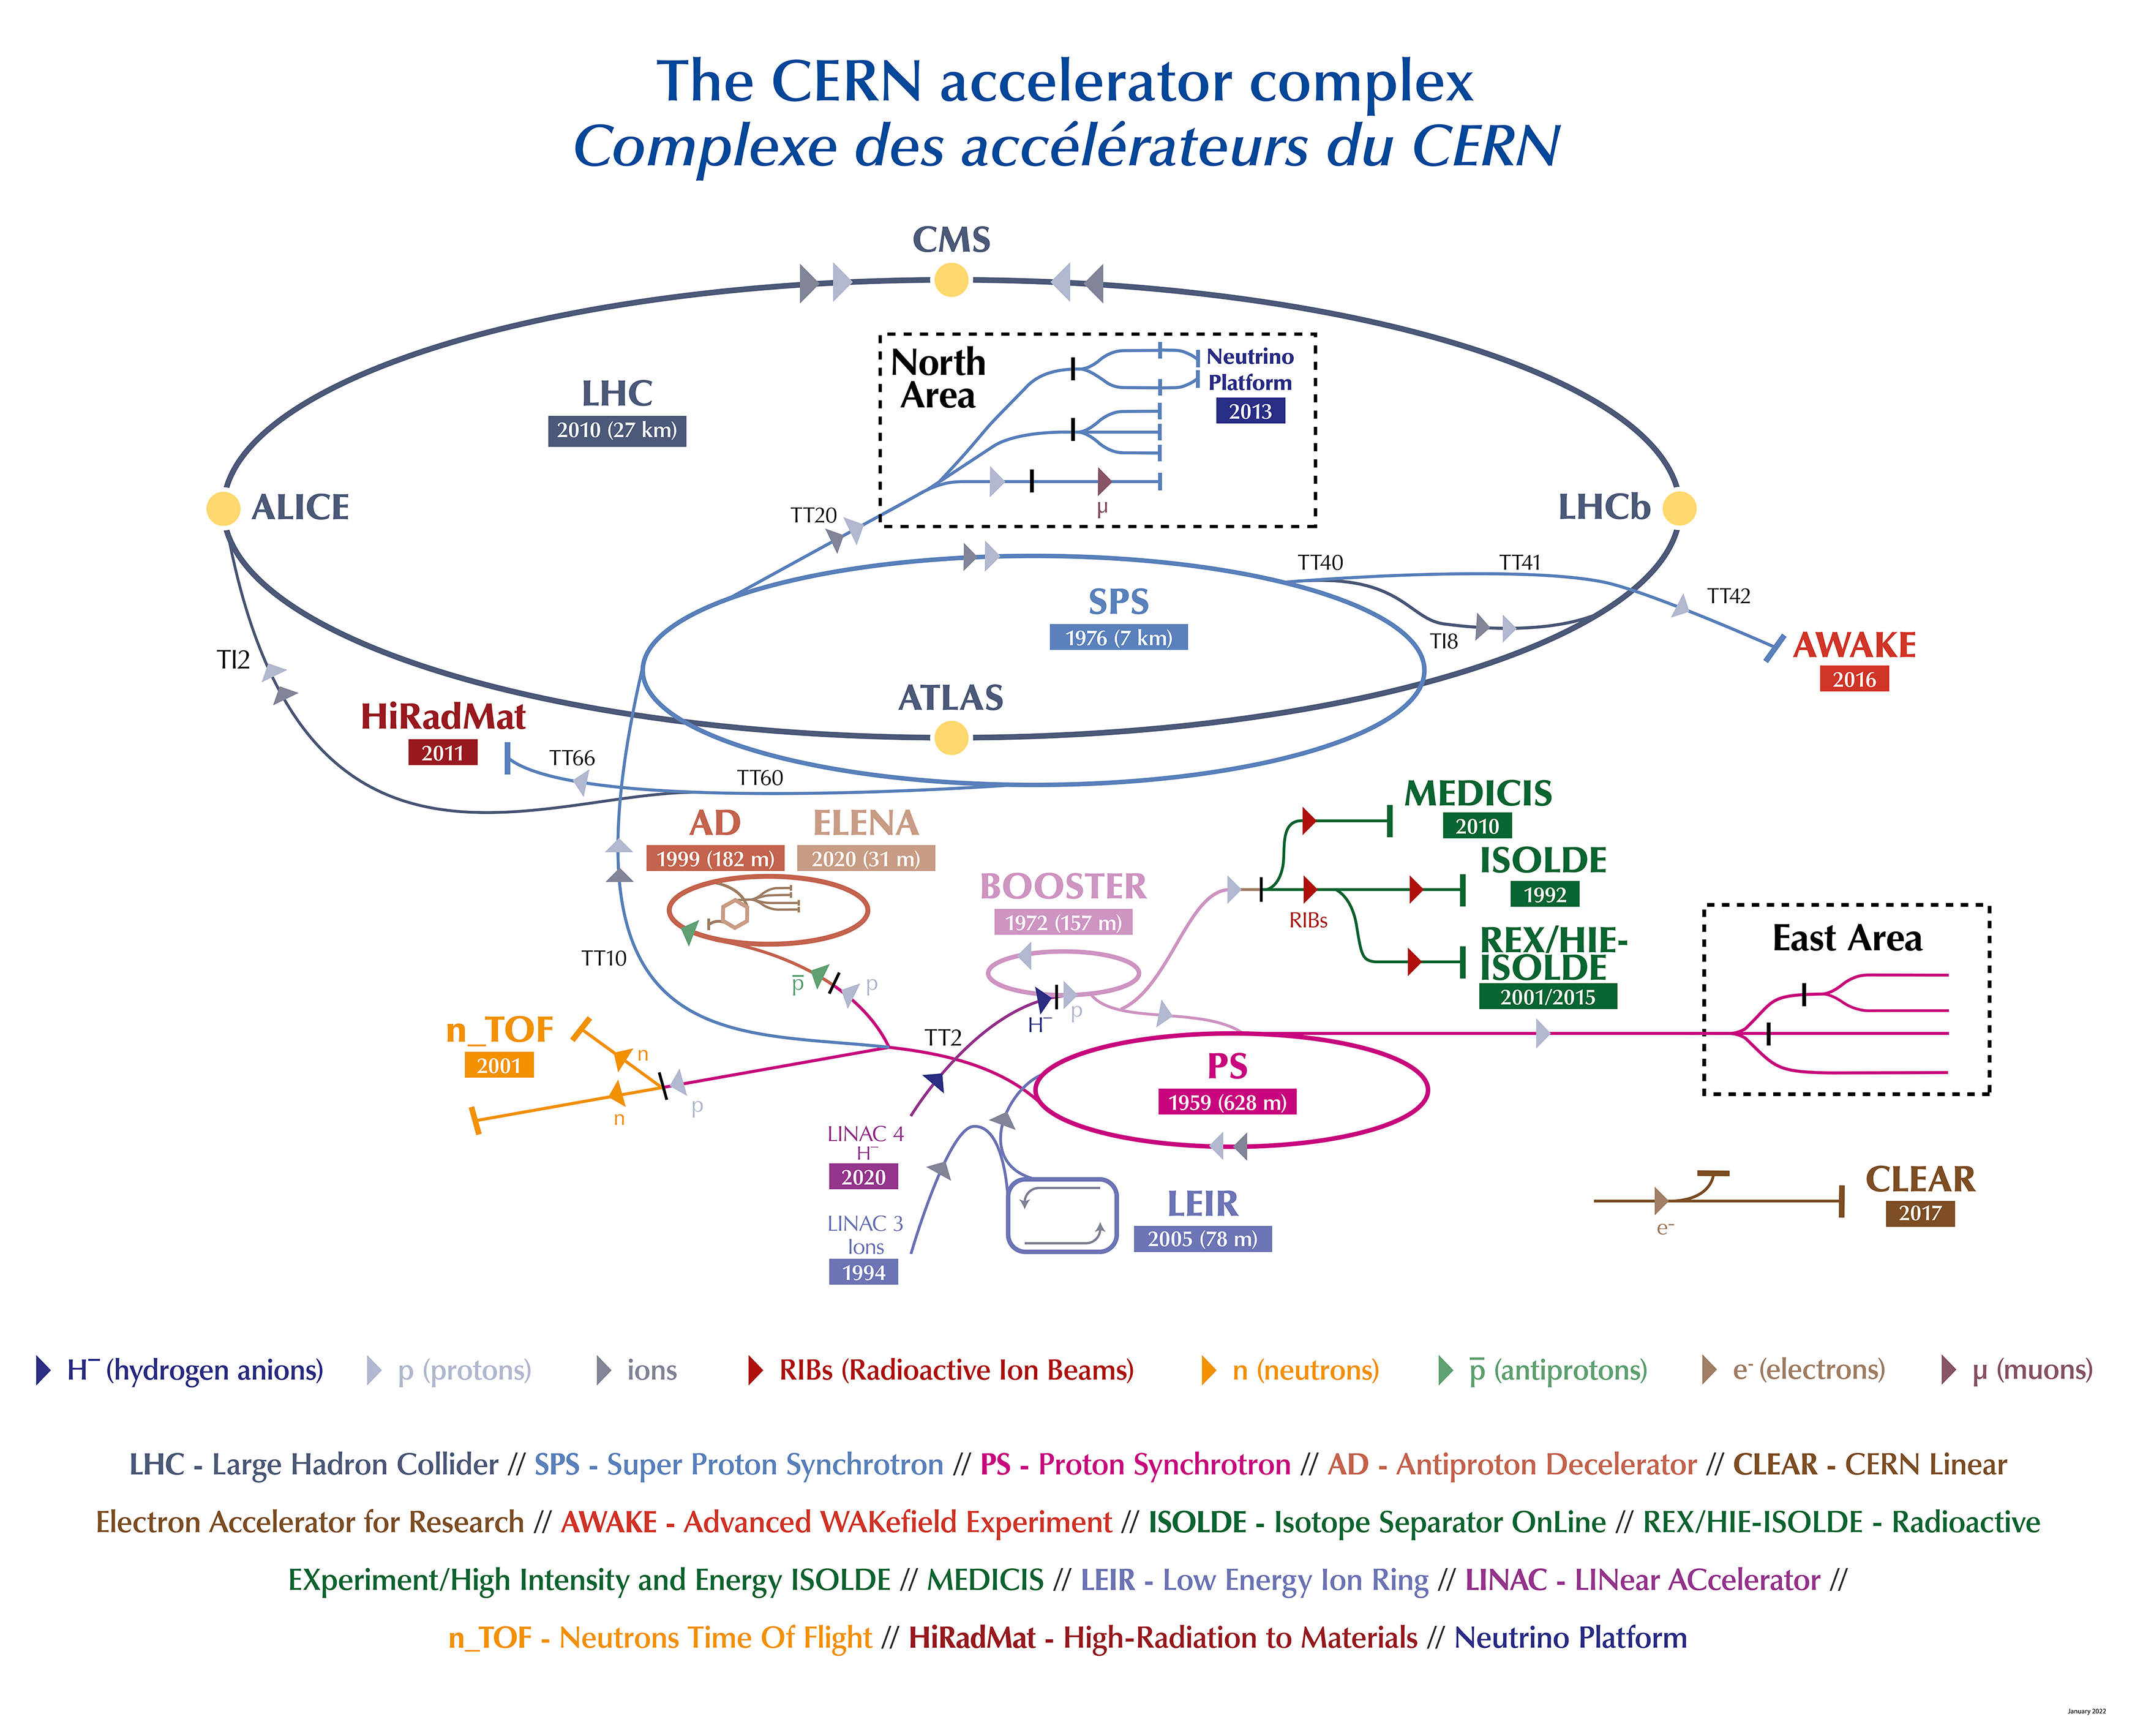
\includegraphics[width=1.0\textwidth]{CCC-v2022-small.png}
        \caption{The CERN accelerator complex, including the Large Hadron Collider (LHC) and its experiments, taken from~\cite{CERNAccComp}}
        \label{fig:LHC}
    \end{figure}

    CERN's early years were marked by the construction of pioneering accelerators, such as the Synchrocyclotron (SC)~\cite{Synchro-CyclotronDivision:1606751}
    in 1957 and the Proton Synchrotron (PS) in 1959~\cite{ADAMS1960}. The SC was CERN's first accelerator, used for nuclear physics 
    experiments, while the PS, with a beam energy of 28 GeV, became instrumental in numerous discoveries, including 
    the observation of neutral currents in 1973. The PS's success laid the groundwork for more advanced facilities 
    and experiments.

    In 1976, the Super Proton Synchrotron (SPS)~\cite{Doble:2312568} began operations, serving both as a particle accelerator and a storage 
    ring. The SPS played a pivotal role in the discovery of the W and Z bosons in 1983, work that earned Carlo Rubbia 
    and Simon van der Meer the Nobel Prize in Physics. These discoveries helped confirm the electroweak theory, a fundamental 
    component of the Standard Model of particle physics.

    The Large Electron-Positron Collider (LEP)~\cite{Schopper:2009zz} was a groundbreaking particle accelerator that operated at CERN from 1989 to 2000. 
    Situated in the same 27-kilometre tunnel that now houses the LHC, LEP was designed to collide electrons and positrons at high 
    energies to probe the fundamental constituents of matter. The construction of LEP was a significant engineering and scientific 
    achievement, involving the development of advanced technologies and large-scale international collaboration. One of the 
    notable accomplishments of LEP was its precision measurements of the Z boson~\cite{ALEPH:2007brf}, which helped to confirm the electroweak theory. 
    The collider's ability to produce clean and precise collisions of electrons and positrons allowed physicists to explore a wide 
    range of phenomena with unprecedented accuracy. Over its 11 years of operation, LEP produced a wealth of scientific results 
    that significantly enhanced our understanding of particle physics and laid the groundwork for future discoveries.

    When LEP was decommissioned in 2000, its tunnel was repurposed for the LHC, which required substantial upgrades to 
    handle the higher energy collisions of protons and heavy ions. 
    The LHC~\cite{Evans:2008zzb}, the most ambitious project at CERN, was officially inaugurated on October 21, 2008. 
    It is designed to collide protons at unprecedented centre-of-mass energy levels, reaching up to 13.6 TeV. The LHC's primary 
    objective is to explore the fundamental properties of matter and the forces governing the universe that beyond the Standard Model.
    The LHC hosts several major experiments, each with specific research goals and sophisticated detection apparatus.
    ATLAS (A Toroidal LHC ApparatuS)~\cite{PERF-2007-01} and CMS (Compact Muon Solenoid)~\cite{CMS-CMS-00-001} are general-purpose detectors. These experiments 
    played a central role in the discovery of the Higgs boson in 2012, a particle essential to the Standard Model as 
    it provides evidence for the mechanism by which other elementary particles acquire mass. 
    The LHCb (Large Hadron Collider beauty)~\cite{LHCb:2008vvz} experiment focuses on investigating the differences between matter and antimatter by studying the decays 
    of particles containing b (beauty) quarks. This research aims to understand why the universe is dominated by 
    matter rather than antimatter, despite the expectation that both should have been produced in equal amounts 
    during the Big Bang.
    ALICE (A Large Ion Collider Experiment)~\cite{ALICE:2008ngc} is designed to study the properties of quark-gluon plasma, a state of matter thought to have existed shortly 
    after the Big Bang. By colliding heavy ions, ALICE aims to recreate and analyse this plasma, providing insights 
    into the strong force that binds quarks and gluons together to form protons and neutrons.
    TOTEM (TOTal Elastic and diffractive cross-section Measurement)~\cite{totem_2008} and LHCf (Large Hadron Collider forward) focus on studying forward particles, 
    those that travel close to the beamline, to gain insights into proton structure and the underlying dynamics of particle collisions. 
    TOTEM measures the total cross-section, elastic scattering, and diffraction processes, while LHCf studies particles produced at very small 
    angles to the beam direction.

    \subsection{The operation of the LHC}
        The LHC's operational phases have significantly advanced particle physics, combining upgrades and high-energy 
        collisions to explore the fundamental aspects of matter and the universe. The ongoing and future upgrades, especially 
        the HL-LHC, promise to further enhance our understanding and potentially lead to groundbreaking discoveries. 
        \subsubsection{Run 1 (2009-2013)}
            Run 1 of the Large Hadron Collider (LHC) at CERN began in 2009 and continued until early 2013. 
            During this period, the LHC operated at proton-proton (p-p) collision energies of 7~TeV (2010-2011) and 8~TeV (2012-2013), 
            laying the groundwork for significant scientific discoveries and establishing the LHC as 
            the world's most powerful particle accelerator. The most notable achievement of Run 1 was the 
            discovery of the Higgs boson~\cite{HIGG-2012-27,CMS-HIG-12-028} in July 2012 by the ATLAS and CMS experiments. This discovery confirmed 
            the last missing component of the Standard Model of particle physics and garnered the 2013 Nobel 
            Prize in Physics for theorists Francois Englert and Peter Higgs. Run 1 also involved extensive searches 
            for new physics beyond the Standard Model, including searches for supersymmetry (SUSY) and extra 
            dimensions, although no definitive evidence was found.
            Lead-lead (Pb-Pb) and proton-lead (p-Pb) collisions were also conducted during Run 1. 
            Run 1 marked the successful commissioning of the LHC's complex systems, including its superconducting magnets, cryogenics, and detectors.
            Significant advancements in data acquisition and analysis techniques were developed, setting the stage for future runs.
        \subsubsection{Long Shutdown 1 (2013-2015)}
            Following the successful completion of Run 1, the LHC entered Long Shutdown 1 (LS1) from early 2013 to early 2015. During this period, 
            significant maintenance and upgrades were carried out to prepare the LHC for higher energy collisions and increased luminosity in 
            subsequent runs. LS1 involved enhancements to the accelerator's magnets, cryogenics, and beam instrumentation, ensuring improved 
            performance and reliability.
        \subsubsection{Run 2 (2015-2018)}
            The LHC resumed operations in 2015 with Run 2. 
            This phase saw the LHC operate at the higher energy of 13 TeV, leading to further significant discoveries 
            and more precise measurements of the Higgs boson and other Standard Model particles~\cite{ParticleDataGroup:2022pth}. 
            The increased energy 
            and luminosity provided new opportunities to search for physics beyond the Standard Model, although no 
            new particles were discovered.
        \subsubsection{Long Shutdown 2 (2019-2021)}
            Following Run 2, the LHC entered Long Shutdown 2 (LS2) for maintenance and upgrades to prepare for even higher 
            luminosity operations. The upgrades aimed to enhance the performance of the accelerator and detectors~\cite{Arduini_2024}, ensuring 
            improved data quality and higher collision rates.
            The COVID-19 pandemic had a notable impact on CERN's LS2. The pandemic necessitated strict health and safety 
            measures, significantly affecting on-site work. CERN implemented remote working protocols and minimised on-site 
            activities to protect staff and contractors. These disruptions caused delays in the planned maintenance and 
            upgrades to the LHC and associated experiments. Despite these challenges, CERN managed to continue essential 
            work, ensuring that critical upgrades were completed, albeit on a postponed schedule. 
        \subsubsection{Run 3 (2022-present)}
            Run 3 began in 2022, operating at 13.6 TeV with further optimised conditions. This phase focuses on collecting 
            more data to enhance the precision of existing measurements and explore new potential discoveries. 
            Operating at higher energy required extensive calibration and tuning of the accelerator 
            components to handle the increased energy and collision rates effectively. Global supply chain issues delayed the delivery of critical components, hindering 
            technical improvements and maintenance work essential for efficient LHC operation during LS2~\cite{Perrot:2845779,covid19_economics}.
            Extensive calibration and validation of upgraded detectors were necessary to ensure accurate and reliable measurements, initially slowing down data collection.
            Despite these challenges, the LHC has ramped up its performance as technical issues are resolved in 2024. The 
            upgraded systems are fully integrated and optimised. In run 3 the LHC has delivered over 160~\ifb of data to the ATLAS and CMS 
            experiments at the time of writing, with 101~\ifb collected in 2024 alone. 

    \subsection{Future LHC upgrades - The High-Luminosity LHC}
        The High-Luminosity Large Hadron Collider (HL-LHC)~\cite{HighLuminosityLHC} is a major upgrade to the current LHC, designed to increase 
        its luminosity by a factor of 5-10. Scheduled to start operations in the late-2020s, the HL-LHC aims to gather 
        approximately 10 times more data than the existing LHC. This significant increase in luminosity will enhance 
        the potential for new discoveries and provide more precise measurements of SM phenomena. 

        The HL-LHC will feature new, stronger superconducting magnets to better focus the proton beams, increasing the luminosity.
        Upgraded cryogenic systems will enhance the cooling power of the accelerator, crucial for maintaining the superconducting state of the magnets.
        The ATLAS, CMS, LHCb, and ALICE detectors will undergo significant enhancements to handle the increased collision 
        rates and data throughput, ensuring they can capture and process the additional information effectively.
        Components will be upgraded to withstand the higher levels of radiation expected from the increased luminosity, 
        ensuring the longevity and reliability of the detector systems.
    
    \subsection{Future collider projects - the Future Circular Collider (FCC)}
        FCC~\cite{Benedikt2020} represents 
        a bold vision for the next generation of particle accelerators, aiming to 
        build upon the discoveries of the HL-LHC. The FCC is a proposed research 
        infrastructure that would significantly extend our understanding of 
        fundamental physics by exploring uncharted energy scales and precision 
        measurements. It is designed to address key questions that remain unanswered 
        in the Standard Model of particle physics and beyond.
        The FCC project encompasses two main collider configurations: the FCC-ee, 
        a high-luminosity electron-positron collider, and the FCC-hh, a high-energy 
        proton-proton collider. The FCC-ee is envisaged as a first step, providing 
        precise measurements of the Higgs boson, W and Z bosons, and the top quark, 
        while the FCC-hh will follow, offering collisions at energies up to 100 TeV, 
        far exceeding the capabilities of the LHC.
        \subsubsection{The FCC-ee: A Precision Machine}
        The FCC-ee collider is designed to operate at various energy stages, initially 
        focusing on Z boson production with centre-of-mass energies around 90 GeV, 
        and subsequently increasing to study the W boson, Higgs boson, and top quark 
        at higher energies. With its unprecedented luminosity and precision, the FCC-ee 
        will provide high-precision measurements of the Higgs boson properties, 
        improved determinations of the W and Z boson masses and couplings, and detailed studies of
        the top quark. The FCC-ee's exceptional precision will allow physicists to probe 
        for tiny deviations from the SM predictions, potentially revealing 
        new physics.
        \subsubsection{The FCC-hh: Exploring the Energy Frontier}
        Following the FCC-ee, the FCC-hh collider aims to push the energy frontier to 
        100 TeV, offering unprecedented opportunities for discovery. The key objectives 
        of the FCC-hh include probing the nature of dark matter by potentially producing 
        dark matter particles through their interactions with SM particles; 
        exploring the Higgs potential and self-interactions to understand the stability 
        of the Higgs field; searching for new particles and forces that could manifest 
        at higher energy scales, providing insights into physics beyond the SM.
        To achieve these goals, the FCC-hh will require significant advancements in 
        technology, including the development of stronger superconducting magnets 
        capable of reaching magnetic fields up to 16~T, and sophisticated detectors 
        designed to handle the higher energy and luminosity.

\section{The ATLAS detector}
    The ATLAS detector~\cite{PERF-2007-01}, installed at Point 1 of the LHC at CERN, 
    is one of the largest and most complex particle detectors ever constructed. A cut-away 
    view of the ATLAS detector in Run 3 configuration is shown in Figure~\ref{fig:ATLAS_cutaway_run3}.
    \begin{figure}[htbp]
        \centering
        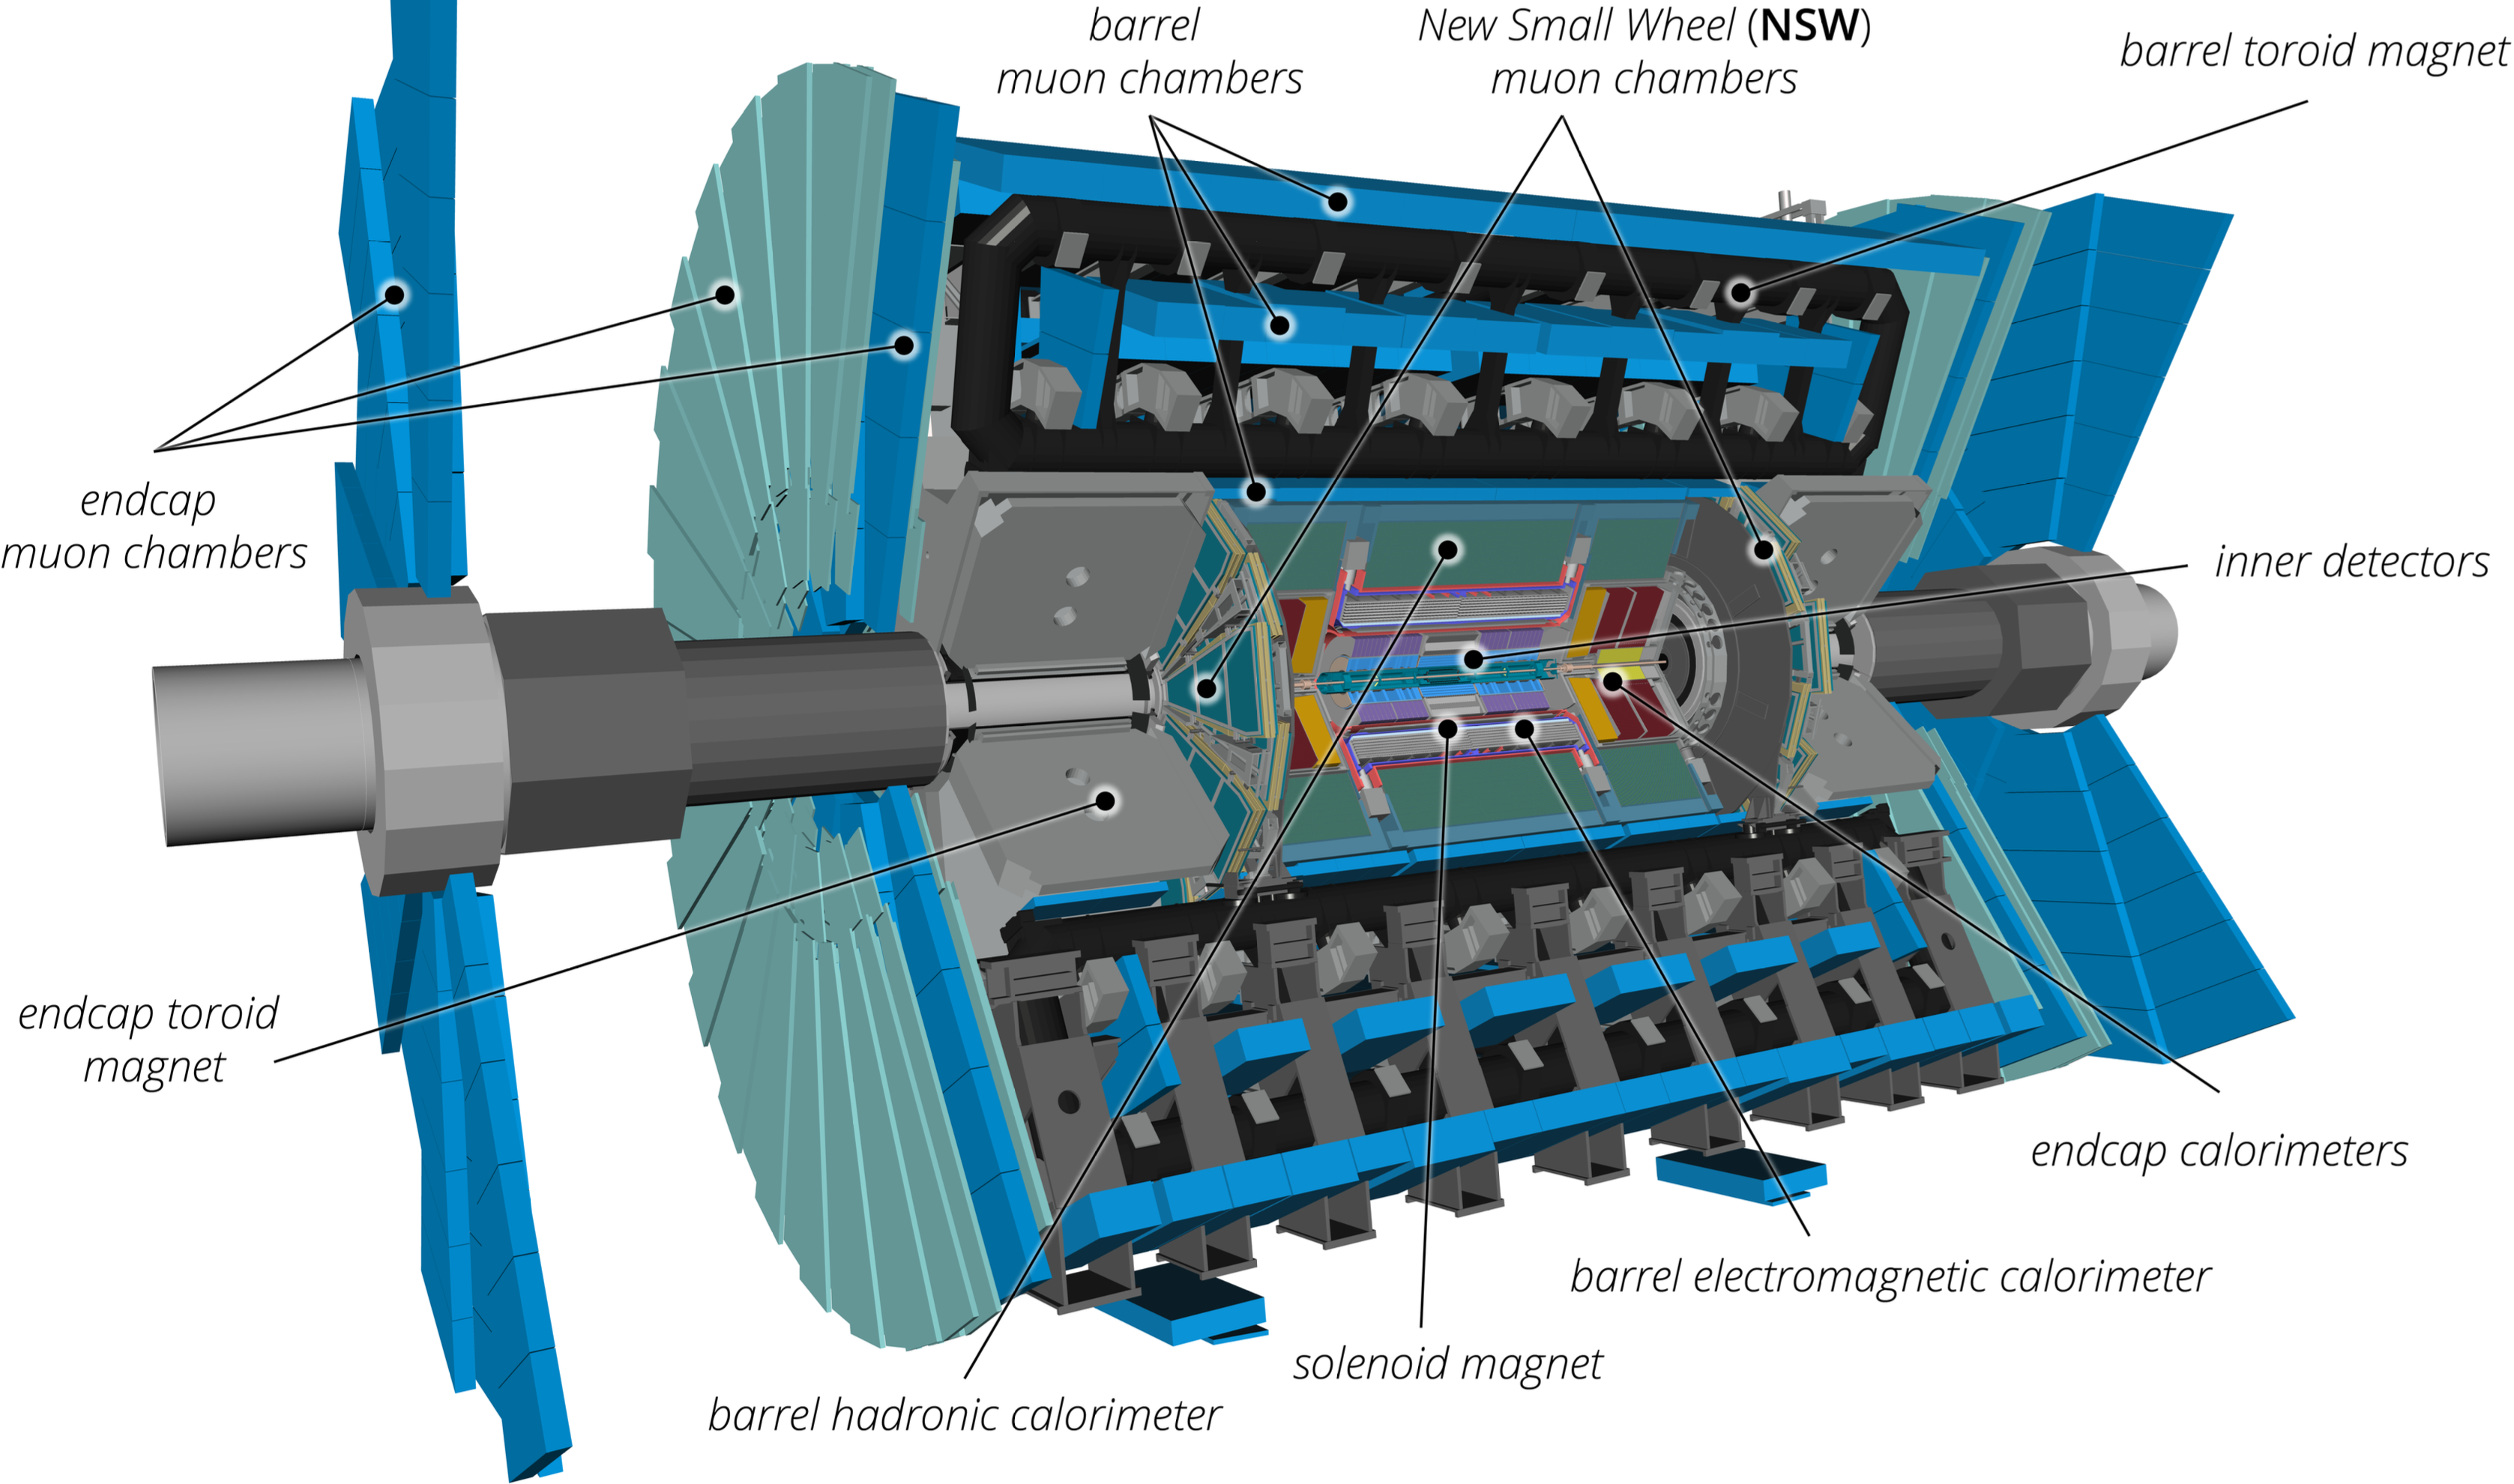
\includegraphics[width=1.0\textwidth]{ATLAS-cutaway-run3.png}
        \caption{Cut-away view of the Run 3 configuration of the ATLAS detector indicating the locations of the larger detector sub-systems, taken from~\cite{GENR-2019-02}}.
        \label{fig:ATLAS_cutaway_run3}
    \end{figure}
    Its diverse array of sophisticated sub-detectors captures and 
    analyses the particles produced in high-energy collisions. The conceptual design of 
    ATLAS began in the early 1990s, with the official Letter of Intent submitted 
    in 1992~\cite{ATLAS-TDR-LOI} and the Technical Proposal in 1994~\cite{ATLAS-TDR-Proposal}. 
    Construction commenced in the late 
    1990s, leading to the installation of the detector in its cavern by 2007. The 
    first proton-proton collisions were recorded in 2009. Over the years, ATLAS has undergone several 
    upgrades to enhance its performance and accommodate increasing collision 
    rates and energies. ATLAS comprises several key components designed to work in concert to achieve 
    comprehensive particle detection and analysis:
    \begin{itemize}
        \item Inner Detector (ID): This component provides precise tracking of charged particle trajectories and interaction points near the collision vertex. It consists of a high-granularity silicon Pixel detector, a Semiconductor Tracker (SCT), and a Transition Radiation Tracker (TRT).
        \item Calorimeters: These measure the energy of particles by absorbing them. The electromagnetic calorimeter detects electrons and photons, while the hadronic calorimeter measures the energy of hadrons. The ATLAS calorimeters use two sampling technologies: liquid argon (LAr) for the electromagnetic calorimeters and all endcap and forward calorimeters, and scintillating tiles for hadron calorimetry in the central region.
        \item Muon Spectrometer: Located outside the calorimeters, this system detects and measures muons, which are minimally ionising particles that penetrate the inner detector and calorimeters. It is based on the magnetic deflection of muon tracks in a large superconducting air-core toroidal magnet system.
        \item Forward Detectors: Comprised of four sub-detectors, the forward detectors play critical roles in measuring luminosity, studying diffractive events, and characterising the centrality~\cite{HION-2010-01} of heavy-ion collisions.
        \item Trigger and Data Acquisition (TDAQ) System: This system selects events of interest based on distinguishing characteristics and reads them out for further offline processing. It consists of the Level-1 Trigger (L1) and the High-Level Trigger (HLT), along with the Data Acquisition system that transports data from sub-detector electronics to offline processing.
    \end{itemize}
    The ATLAS detector has been continuously upgraded to maintain its performance under the increasingly challenging 
    conditions of the LHC. The Phase-I upgrades~\cite{ATLAS-TDR-20,ATLAS-TDR-22,ATLAS-TDR-23,ATLAS-TDR-24}, 
    implemented during LS2 from 2019 to 2022, included improvements to the detector subsystems and their electronics to withstand the high interaction rates expected 
    in Run 3 and beyond. These upgrades focused on enhancing the trigger system, increasing precision tracking, 
    and improving calorimetry and muon detection capabilities. In recent years, the LHC has achieved higher collision 
    energies and luminosities, necessitating further upgrades to the ATLAS detector. 
    The Run 3 configuration, for example, includes new LAr Calorimeter digital trigger electronics, 
    an upgraded Muon Spectrometer with new small wheels (NSWs), and enhanced TDAQ systems to handle the increased data rates and complexity. 
    The Phase-II upgrades, planned for the HL-LHC era~\cite{ATLAS-TDR-PhaseII,ATLAS-TDR-25,ATLAS-TDR-26,ATLAS-TDR-27,ATLAS-TDR-28,ATLAS-TDR-29,ATLAS-TDR-30,ATLAS-TDR-31}, 
    will further enhance the detector's capabilities to meet the demands of higher luminosities and energies. 
    These upgrades will include 
    improvements in calorimeters for higher granularity and faster readout electronics to handle higher collision rates,
    a complete replacement of the ID (ITK) that can handle 
    the increased pile-up conditions and radiation dose,
    upgrades to the TDAQ system that can handle date rates up to 1~MHz at Level-0 and 400~kHz at Level-1,
    and an upgraded Muon Spectrometer for better coverage and resolution. 
    In the following sections, we will delve into the key components of the ATLAS detector
    and their functions in particle detection and analysis. 

    \subsection{ATLAS Coordinate System and Kinematic Variables}
        ATLAS uses a right-handed coordinate system with its origin at the nominal 
        interaction point (IP) in the centre of the detector. The axes are defined as follows:
        the z-axis points along the beamline.
        The x-axis points from the IP to the centre of the LHC ring. 
        The y-axis points upwards, perpendicular to the xz-plane.
        Cylindrical coordinates $(r, \phi)$ are used in the transverse plane, where $r$ is the radial 
        distance from the z-axis, and $\phi$ is the azimuthal angle around the z-axis. 
        In hadron-hadron collisions, rapidity ($y$) 
        and pseudorapidity ($\eta$) are used to describe the angle of a particle relative to the beam axis.
        $y$ is defined as:
        \[
        y = \frac{1}{2} \ln \left( \frac{E + p_z}{E - p_z} \right),
        \]
        where \( E \) is the energy of the particle, and \( p_z \) is the component of the momentum along the beam axis.
        $y$ is advantageous because differences in $y$ are invariant under Lorentz 
        boosts along the z-axis, making it a particularly useful variable in hadron collider physics.
        $\eta$ is a simplified version of $y$, used when the particle mass is negligible compared to its momentum. 
        It is defined as:
        \[
        \eta = -\ln \left( \tan \frac{\theta}{2} \right),
        \]
        where \( \theta \) is the polar angle with respect to the beam axis. 
        $\eta$ is commonly used in collider experiments to describe the angular distribution of particles because it is 
        a more convenient variable than $y$ due to its simpler form, and the fact that it is approximately equal to $y$ 
        for relativistic particles.
        The trajectory of a particle is typically described in terms of its transverse momentum (\pt), $\phi$, $\eta$. 
        $\pt$ is particularly important in collider physics because it is invariant under 
        boosts along the beam axis, and it is conserved in particle collisions. It is defined as:
        \[
        \pt = \sqrt{p_x^2 + p_y^2},
        \]
        where \( p_x \) and \( p_y \) are the momentum components in the transverse plane.

    \subsection{Inner Detector}
        The Inner Detector (ID)~\cite{IDET-2010-01,IDET-2013-01,IDET-2015-01} of the ATLAS experiment 
        is a sophisticated component designed to provide 
        precise tracking of charged particles originating from the collisions. A cut-away view of the
        ATLAS Inner Detector is shown in Figure~\ref{fig:ID_cutaway}.
        \begin{figure}[htbp]
            \centering
            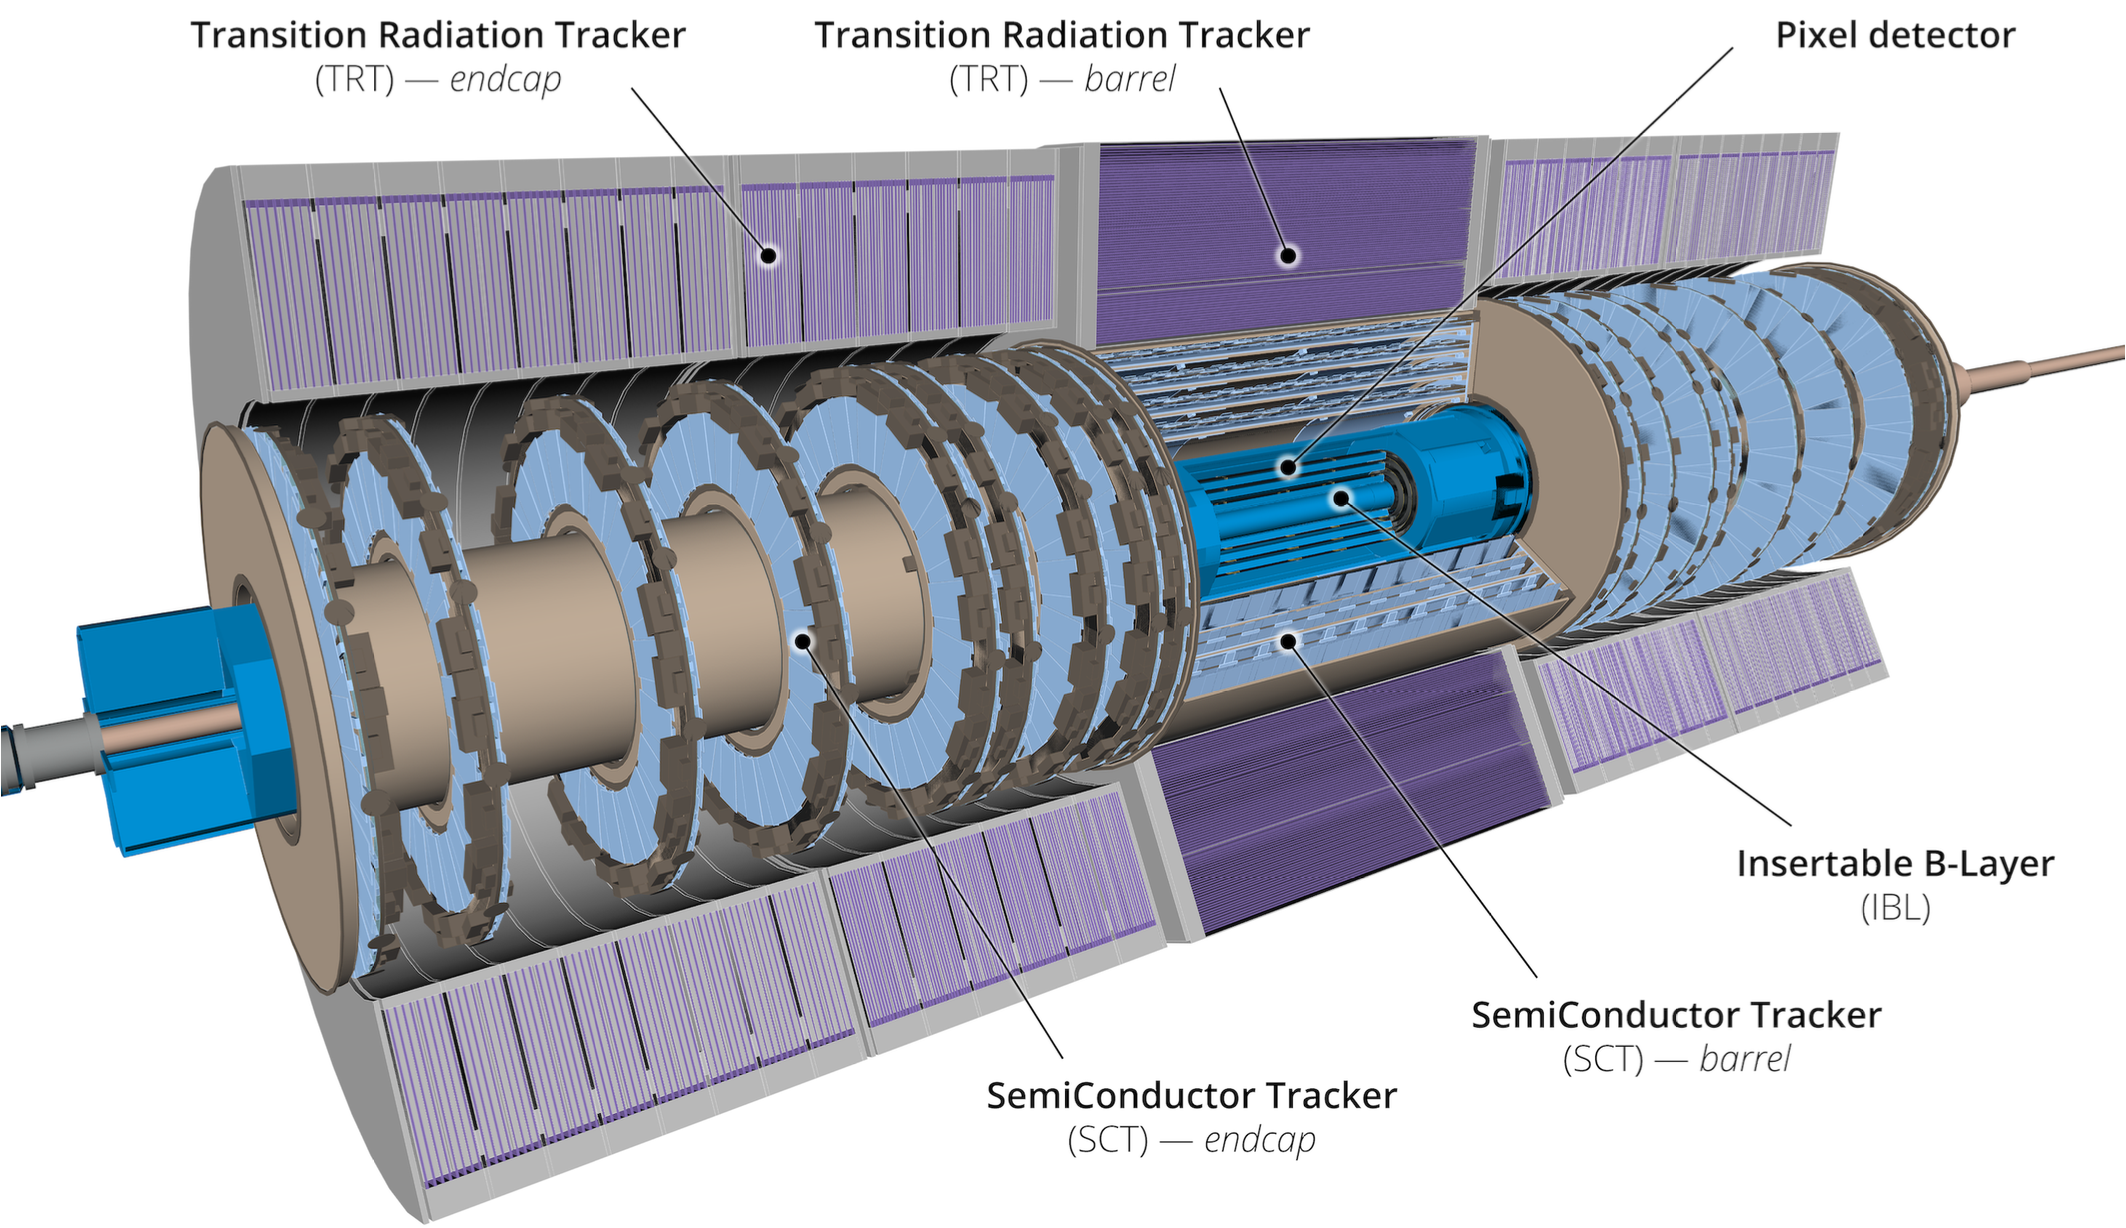
\includegraphics[width=1.0\textwidth]{ATLAS-ID-run3.png}
            \caption{Cut-away view of the ATLAS Inner Detector showing the Pixel Detector, 
                Semiconductor Tracker (SCT), and Transition Radiation Tracker (TRT), taken from~\cite{GENR-2019-02}.}
            \label{fig:ID_cutaway}
        \end{figure}
        The ID is crucial for reconstructing particle trajectories, measuring momenta, and identifying primary and 
        secondary vertices. The design and configuration of the ID have evolved to meet the increasing 
        demands of the LHC. Higher pile-up conditions and radiation levels expected in Run 2 and Run 3
        have necessitated upgrades to the ID to maintain its performance and reliability.
    
        The ID is immersed in a 2~T axial magnetic field generated by a central solenoid, 
        extending over a length of 5.3 meters with a diameter of 2.5 meters~\cite{ATLAS-TDR-06}. The ID covers the 
        pseudorapidity range $|\eta| < 2.5$ and is composed of three primary sub-systems: 
        the Pixel Detector, 
        the Semiconductor Tracker (SCT), 
        and the Transition Radiation Tracker (TRT).
        \begin{itemize}
            \item Pixel Detector~\cite{ATLAS-TDR-11}: The Pixel Detector provides the highest granularity tracking close to the 
            interaction point. It consists of three barrel layers and three endcap discs on each side, with an 
            additional fourth inner layer known as the Insertable B-Layer (IBL)~\cite{PIX-2018-001} installed during LS1. 
            The pixels have dimensions of $50~\si{\um} \times 400~\si{\um}$, 
            with the IBL featuring even finer segmentation at $50~\si{\um} \times 250~\si{\um}$. 
            This system typically provides four precise position 
            measurements per track, aiding in pattern recognition, accurate vertex reconstruction and b-tagging.
            \item Semiconductor Tracker (SCT)~\cite{SCTD-2019-01}: Surrounding the Pixel Detector, the SCT extends the tracking 
            capabilities further from the interaction point. It consists of four barrel layers and nine endcap 
            discs on each side. The SCT uses silicon microstrip technology, with strips oriented to measure both 
            radial and azimuthal coordinates, providing eight measurements per track. The strip pitch is approximately 
            80~$\si{\um}$, allowing for high-resolution tracking over a larger volume than the Pixel Detector.
            \item Transition Radiation Tracker (TRT)~\cite{IDET-2015-01}: The outermost component of the ID, the TRT,
            consists of layers of straw tubes interleaved with radiators that induce transition radiation 
            when traversed by high-energy electrons. The TRT covers range $|\eta| < 2.0$, offering additional particle identification 
            capabilities through the measurement of energy deposition in the straws.
        \end{itemize}
        Several upgrades and enhancements have been implemented in the ID for Run 3 to handle the increased 
        collision energy of 13.6 TeV and the higher luminosity conditions. These include improvements in 
        detector readout electronics, data acquisition systems, and the integration of new cooling systems 
        to maintain optimal operational conditions under the high-radiation environment anticipated during Run 3.
        The precision tracking performance of the ID has been pivotal in enabling ATLAS to achieve its broad 
        physics objectives, from detailed studies of the Higgs boson to searches for new physics phenomena. 
        \begin{figure}[htbp]
            \centering
            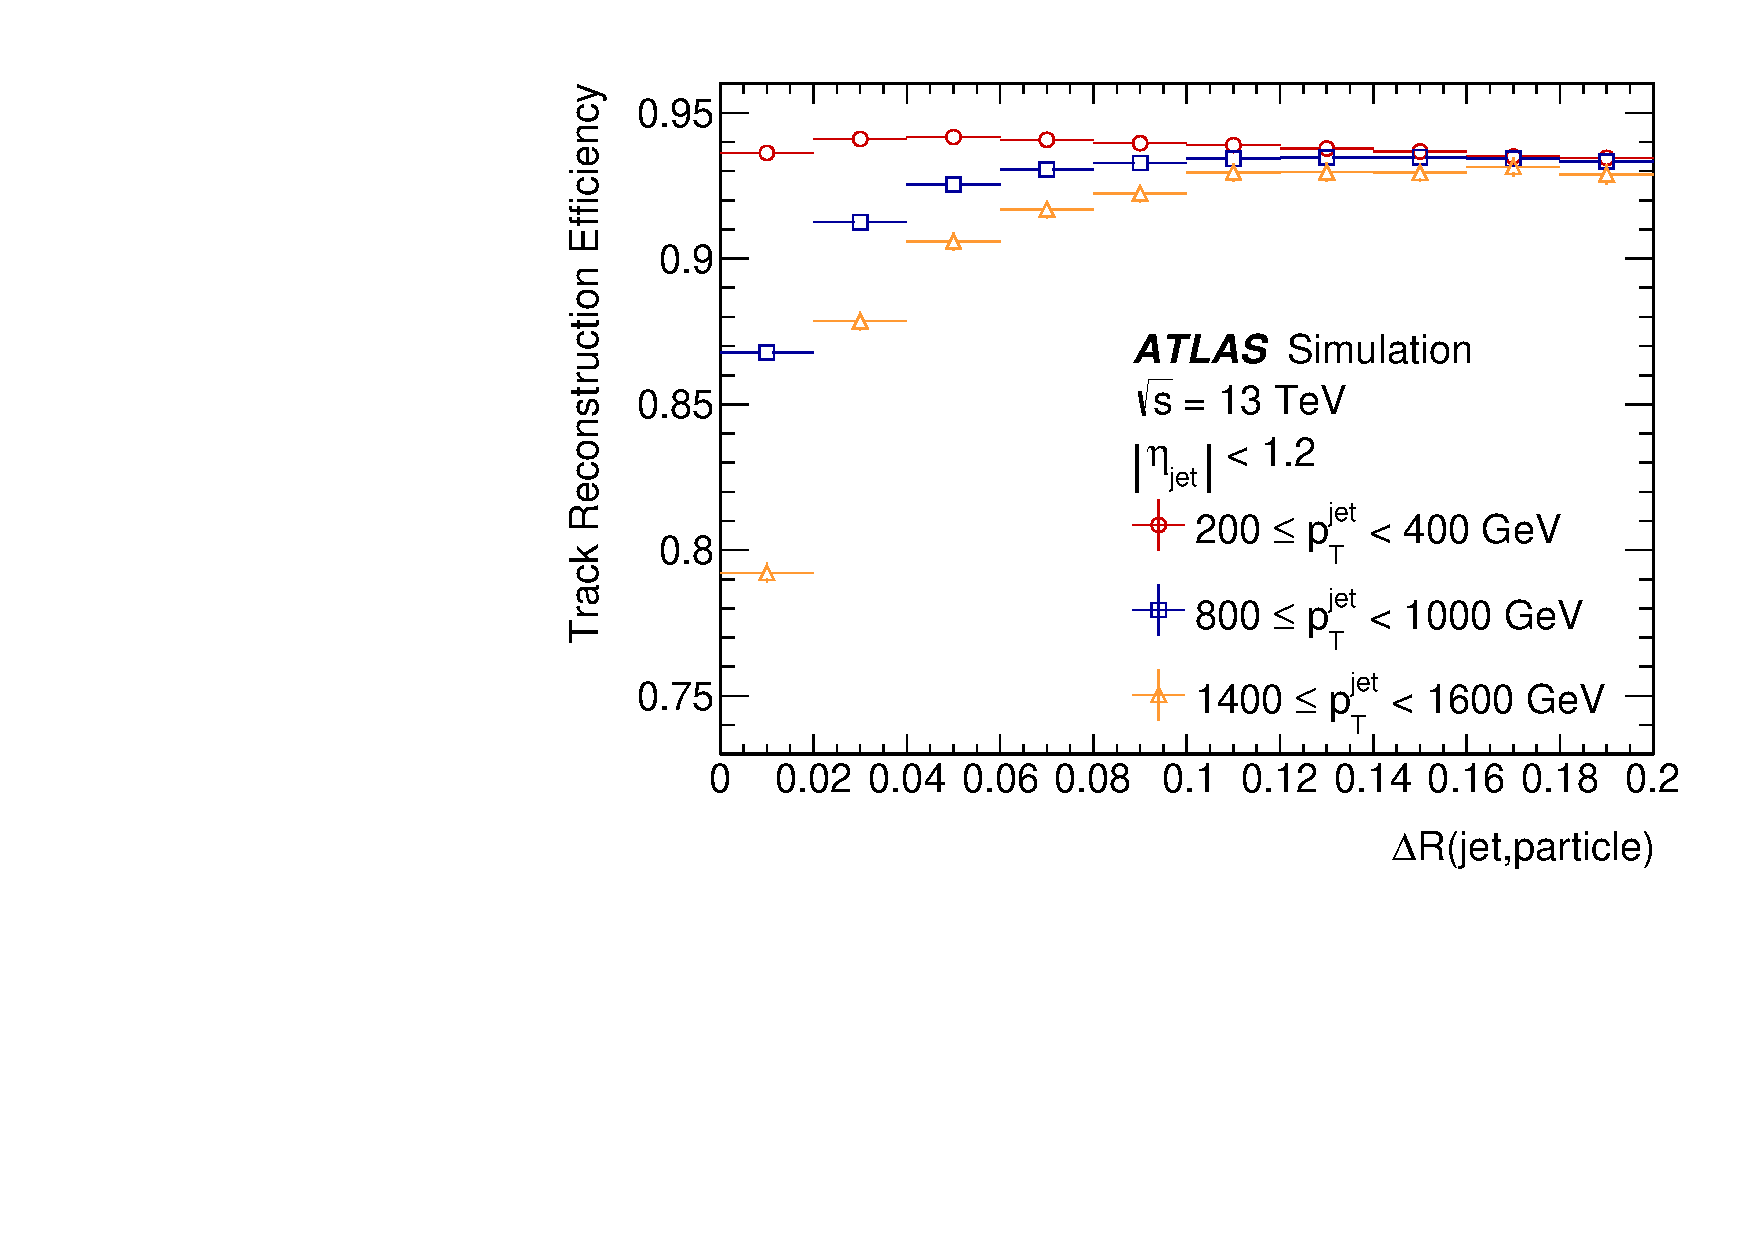
\includegraphics[width=0.495\textwidth]{trk_eff_loeta.pdf}
            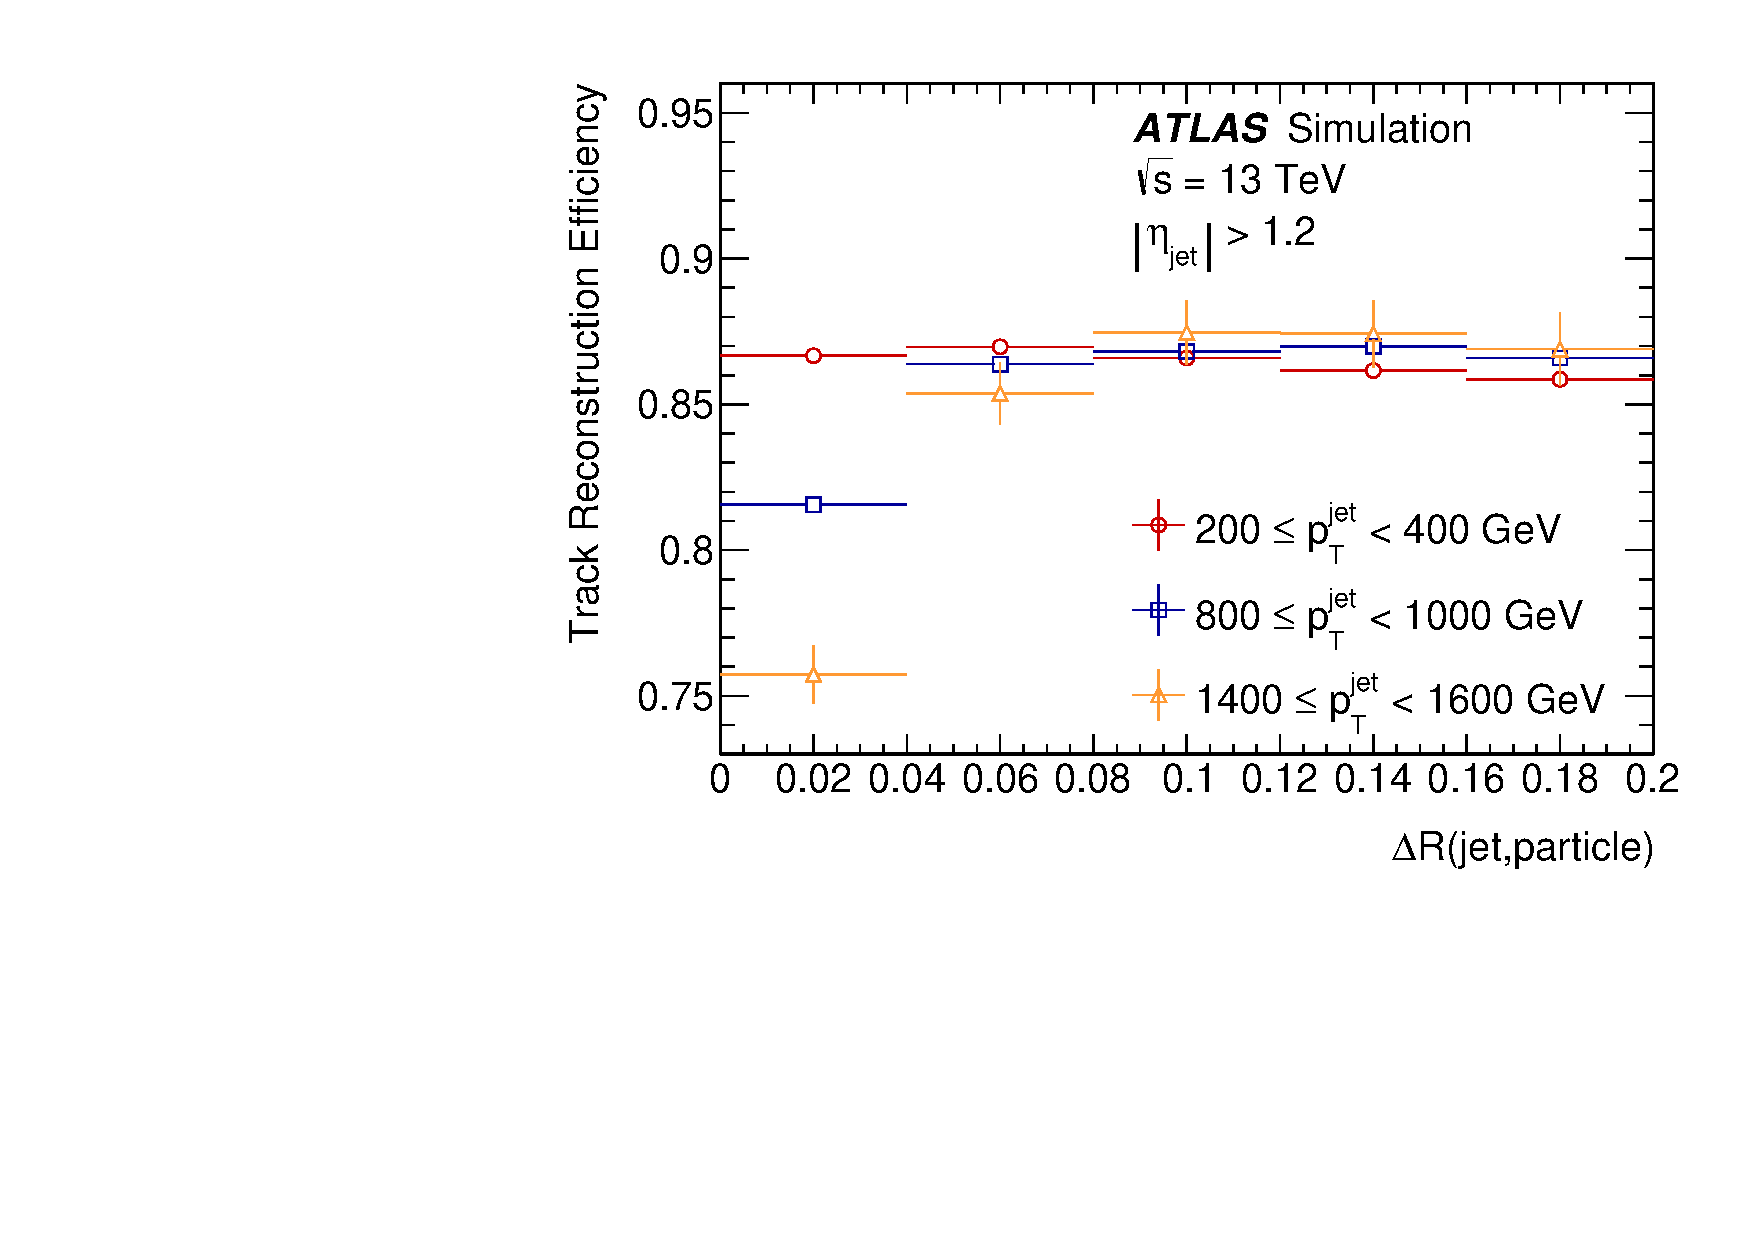
\includegraphics[width=0.495\textwidth]{trk_eff_hieta.pdf}
            \caption{
                The efficiency to reconstruct charged primary particles in jets with (left) $|\eta|< 1.2$ and (right) $|\eta|> 1.2$ is
                shown as a function of the angular distance of the particle from the jet axis for various jet $\pt$ for simulated dijet
                MC events. These figures are taken from~\cite{PERF-2015-08}.
            }
            \label{fig:trk_eff}
        \end{figure}
    \subsection{Calorimeters}
        The ATLAS calorimeter system measures the energies and positions of charged and
        neutral particles through interleaved absorber and active layers out to $|\eta| < 4.9$.
        The calorimeter system is divided into two main types of calorimeters: 
        the Liquid Argon~(LAr)~\cite{ATLAS-TDR-02} calorimeters and the 
        Tile calorimeters~\cite{ATLAS-TDR-03}, each optimised for different aspects of calorimetry.
        A cut-away view of the ATLAS calorimeter system is shown in Figure~\ref{fig:Calo_cutaway}.
        \begin{figure}[htbp]
            \centering
            \includegraphics[width=1.0\textwidth]{ATLAS-calo-run3.png}
            \caption{Cut-away view of the ATLAS calorimeter system showing the Liquid Argon (LAr) 
                calorimeters and the Tile calorimeters, taken from~\cite{GENR-2019-02}.}
            \label{fig:Calo_cutaway}
        \end{figure}
        \subsubsection{Liquid Argon Calorimeters}
            The Liquid Argon (LAr) calorimeter systems are responsible for high-precision measurements 
            of the energy deposited by electrons, photons, and hadrons. 
            They employ a sampling technology, where layers of absorbing material are 
            interleaved with active liquid argon layers. This design allows the calorimeters to measure 
            the energy of particles by sampling their energy loss as they pass through the detector.
            It is divided into several subsystems, each serving a specific purpose:
            \begin{itemize}
            \item LAr Electromagnetic Barrel Calorimeter (EMB): this subsystem covers the central region of the detector and is designed to measure the energy of electrons and photons with high precision. The EMB uses lead absorbers and liquid argon as the active medium.
            \item LAr Electromagnetic Endcap Calorimeter (EMEC): extending the coverage to the forward regions, the EMEC provides similar functionality to the EMB but for particles emitted at smaller angles relative to the beamline.
            \item LAr Hadronic Endcap Calorimeter (HEC): located behind the EMEC, the HEC measures the energy of hadrons. It uses copper absorbers and liquid argon, providing complementary measurements to the Tile calorimeters in the central region.
            \item LAr Forward Calorimeter (FCal): positioned in the very forward regions, the FCal is designed to measure the energy of particles at small angles to the beamline, using a combination of tungsten and liquid argon.
            \end{itemize}

        \subsubsection{Tile Calorimeters}
            The Tile calorimeter system is designed to measure the energy of hadrons and jets in the central 
            region of the detector. It consists of steel absorbers interleaved with scintillating tiles. 
            The Tile calorimeter is segmented into three barrel structures. 
            The Central Barrel (CB) covers the central region around the interaction point and the Extended
            Barrels (EB), positioned on either side of the central barrel to extend the coverage.
            The Tile calorimeter also uses a sampling technique, with the scintillating tiles producing light when 
            charged particles pass through them. This light is then collected by photomultiplier tubes (PMTs) and 
            converted into electronic signals that are processed to determine the energy of the incident particles.
        \subsubsection{Calorimeter Upgrades for Run 3}
            The ATLAS calorimeter system has undergone significant upgrades to enhance its performance for Run 3~\cite{ATLAS-TDR-22}. 
            These upgrades include improvements to the readout electronics and the implementation of a new digital 
            trigger system for the LAr calorimeters. These enhancements are aimed at handling the higher collision 
            energy and increased luminosity expected during Run 3, ensuring that the calorimeter system continues 
            to provide precise measurements under more demanding conditions.
            The calorimeters are critical for a wide range of physics analyses, including the identification and measurement 
            of electrons, photons, taus, and jets, as well as the calculation of missing transverse energy (\MET). 
    \subsection{Muon Spectrometer}
        The ATLAS Muon Spectrometer (MS)~\cite{ATLAS-TDR-10} forms the large outer part of the ATLAS detector, designed 
        to detect charged particles exiting the barrel and endcap calorimeters in the pseudorapidity range \(|\eta| < 2.7\). 
        The primary goal of the MS is to 
        provide precise momentum measurements and trigger capabilities for muons. A cut-away view of the
        ATLAS Muon Spectrometer is shown in Figure~\ref{fig:MS_cutaway}.
        \begin{figure}[htbp]
            \centering
            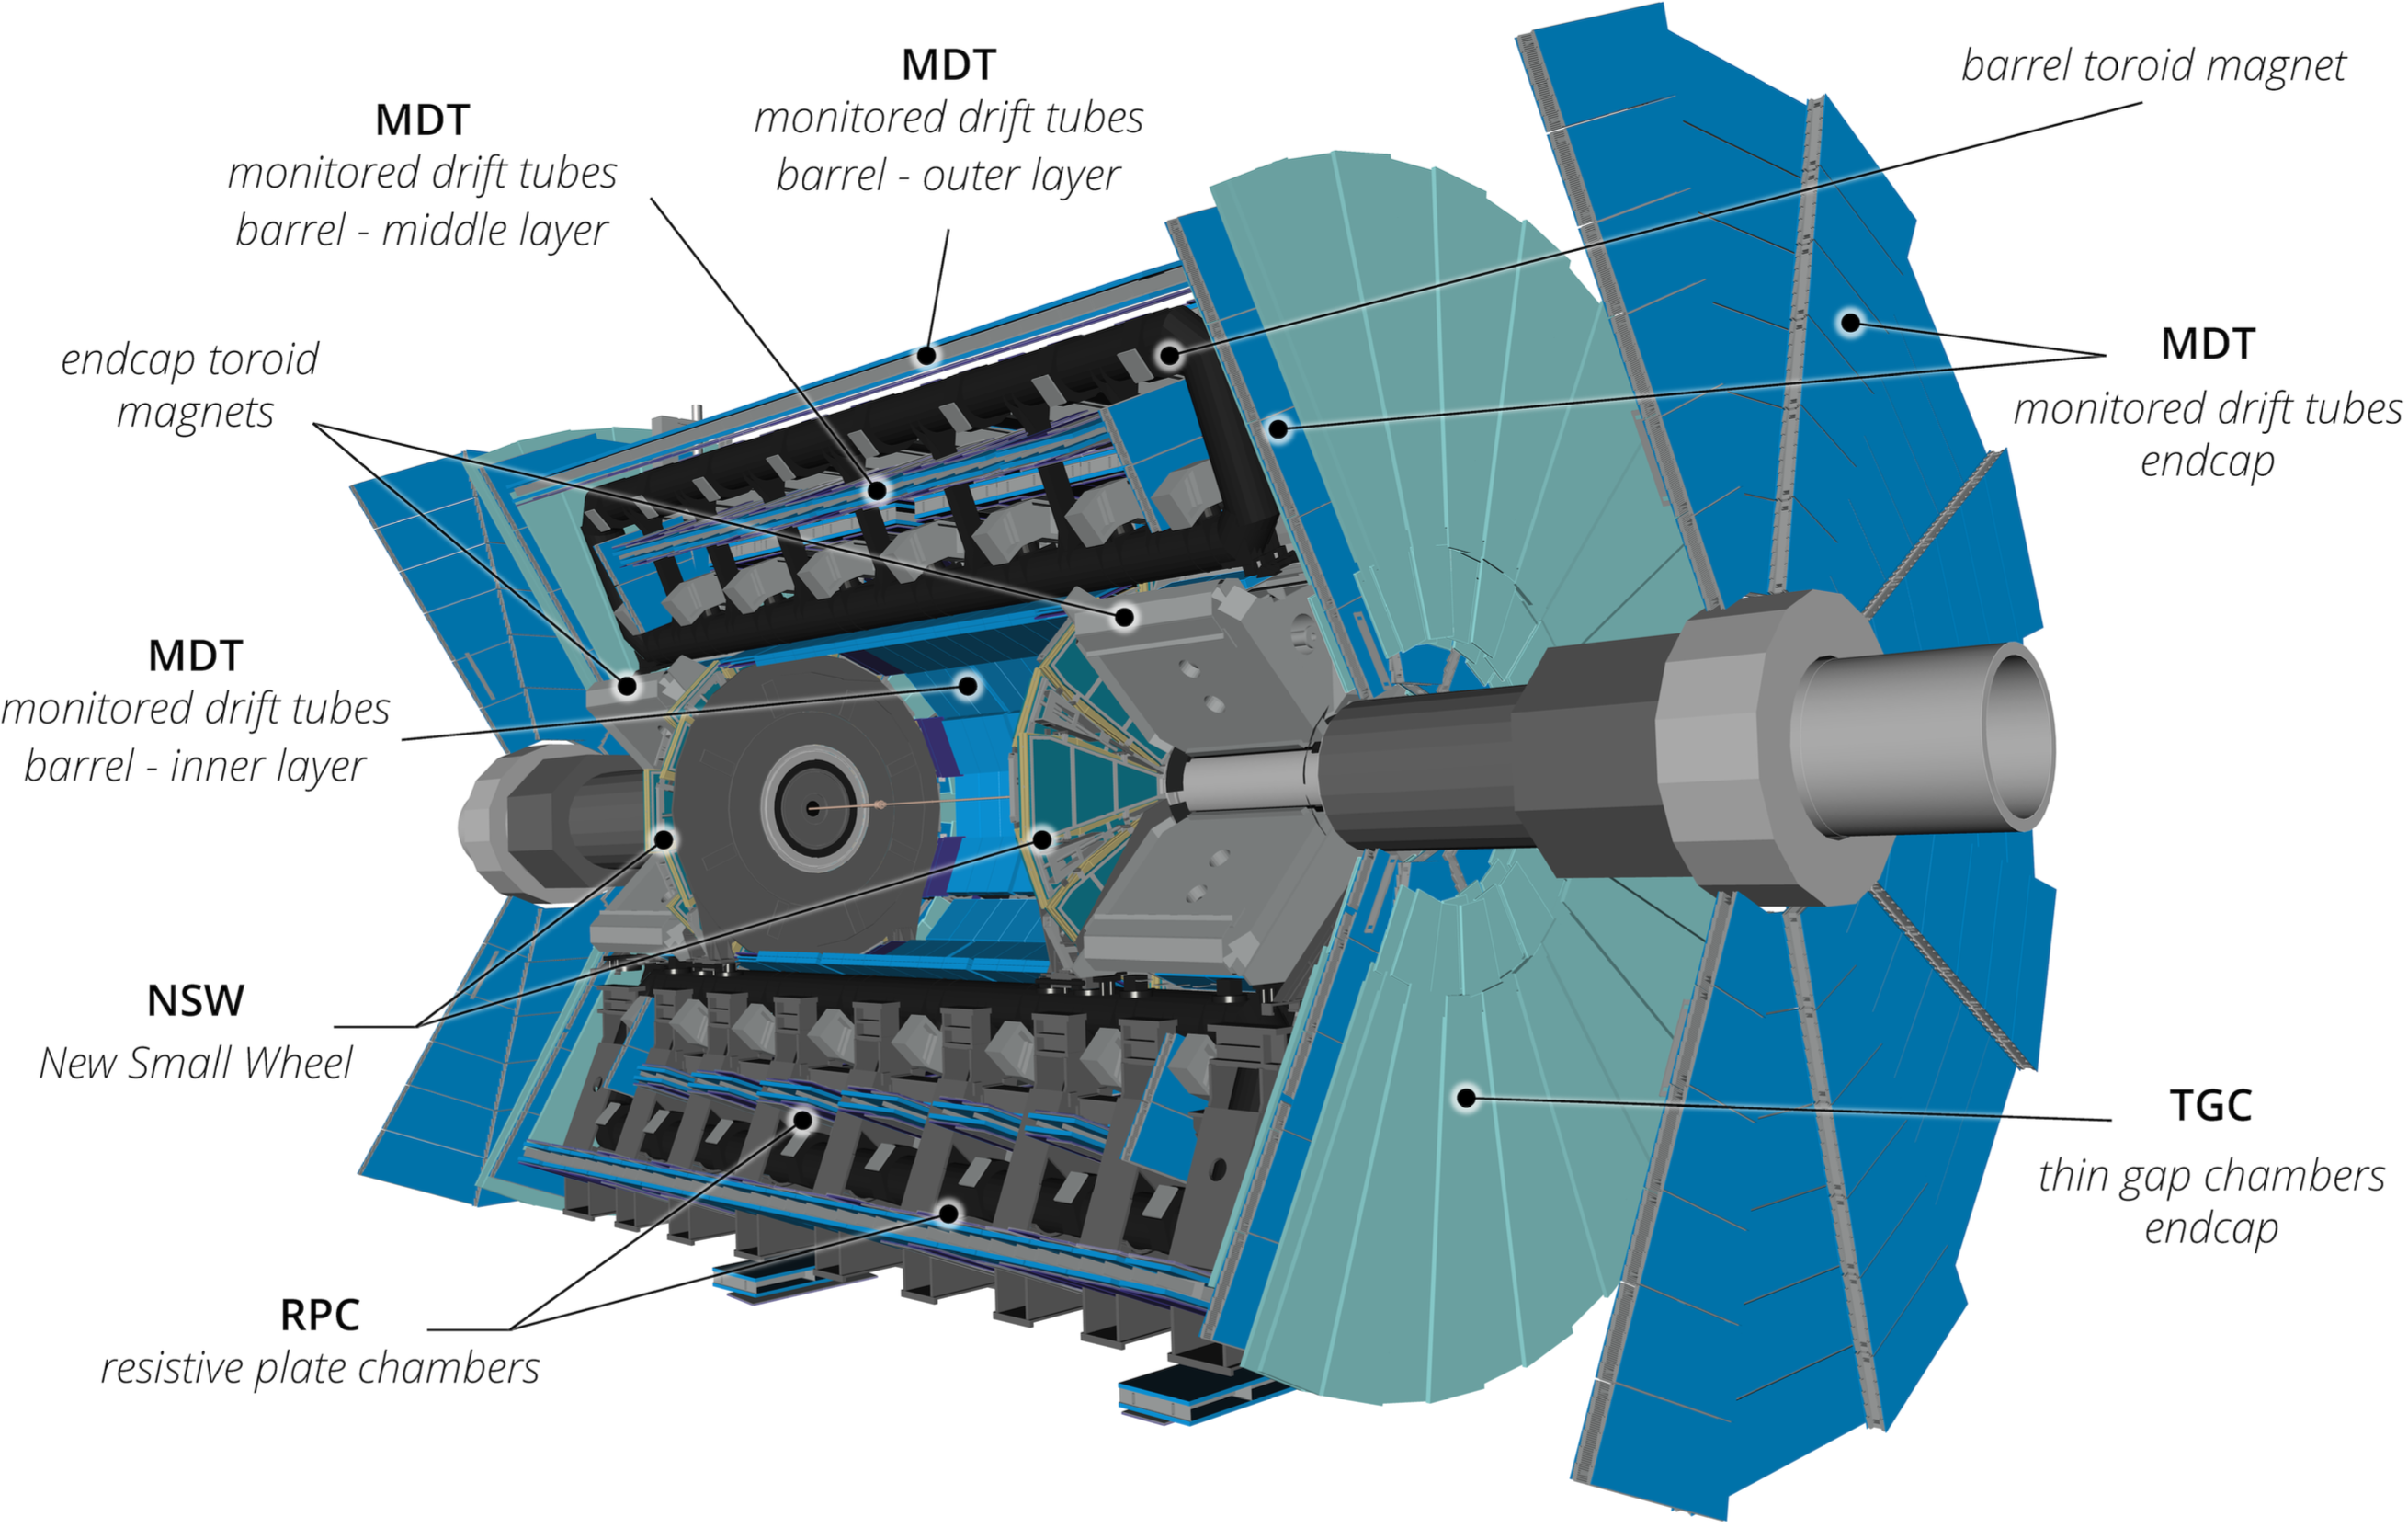
\includegraphics[width=1.0\textwidth]{ATLAS-MS-run3.png}
            \caption{Cut-away view of the ATLAS Muon Spectrometer, taken from~\cite{GENR-2019-02}.}
            \label{fig:MS_cutaway}
        \end{figure}

        The MS is composed of several layers of different detector technologies, all optimised for 
        tracking muons through the strong magnetic fields generated by the ATLAS toroidal magnet system. 
        The MS is divided into three main regions: the barrel, the endcaps, and the transition regions 
        between the barrel and endcaps.
        \begin{itemize}
        \item Barrel Region: the barrel region covers the central part of the detector (\(|\eta| < 1.0\)) and consists of three concentric cylindrical layers known as stations. These stations are equipped with Monitored Drift Tubes (MDTs) for precision tracking and Resistive Plate Chambers (RPCs) for triggering.
        \item Endcap Regions: the endcaps extend the coverage of the MS to higher pseudorapidities (\(1.0 <|\eta| < 2.7\)). Each endcap consists of three disc-shaped stations. The precision tracking in the endcaps is provided by MDTs and Cathode Strip Chambers (CSCs), while the triggering is primarily handled by Thin Gap Chambers (TGCs).
        \item Transition Regions: these regions (\(1.0 < |\eta| < 1.4\)) require special treatment due to the overlap of the barrel and endcap magnetic fields. 
        \item New Small Wheels (NSWs)~\cite{ATLAS-TDR-20}: equipped with Small-Strip Thin Gap Chambers (sTGCs) and Micromegas detectors, the NSWs improve the resolution and redundancy in the $1.3 < |\eta| < 2.7$ region.
        \end{itemize}
        The MDTs are the primary technology used for precision tracking within the MS. Each MDT chamber 
        contains multiple layers of drift tubes, which measure the time taken for ionisation electrons 
        produced by a traversing muon to reach a central wire. This time measurement allows for precise 
        determination of the muon's trajectory. MDTs cover the entire pseudorapidity range of the MS 
        up to \(|\eta| = 2.7\), providing high-resolution tracking data.
        RPCs are used in the barrel region for fast muon triggering. They consist of two parallel plates 
        with a high voltage applied across them. When a muon passes through the chamber, it ionises the 
        gas between the plates, creating an electrical signal that is detected and used to generate a 
        trigger. RPCs also provide measurements of the azimuthal coordinate of muon tracks, aiding 
        in the overall reconstruction process.
        TGCs are used in the endcaps for both triggering and precision tracking. Similar to RPCs, 
        TGCs operate by detecting ionisation events caused by traversing muons. They are designed to 
        handle the high particle fluxes present in the endcap regions and are essential for providing 
        rapid trigger signals to the data acquisition system.    
        CSCs are employed in the innermost endcap layers where particle fluxes are highest. They 
        consist of a plane of wires sandwiched between cathode strips. When a muon passes through 
        the chamber, it ionises the gas, and the resulting electrons are collected by the wires, 
        while the ions induce a signal on the cathode strips. This configuration allows for precise 
        two-dimensional tracking.
        The NSWs, installed as part of the Phase-I upgrades, are designed to handle the high particle 
        rates and provide improved precision in the forward region. They utilise two types of 
        detectors: sTGCs and Micromegas. The sTGCs offer fast response times for triggering, while 
        the Micromegas provide high spatial resolution for tracking. The combination of these 
        technologies ensures robust performance in the high-radiation environment expected during Run 
        3 and beyond.
        The MS aims for a stand-alone transverse momentum resolution better than 15\% for 1 TeV tracks, 
        which requires an effective sagitta resolution of about 75 \(\mu\)m over a large detector volume. 
        This precision is achieved through careful design and regular upgrades. For Run 3, the MS has 
        undergone significant enhancements, in addition to NSWs, the MDT readout electronics has been upgraded
        to handle higher data rates and improve overall performance.
        \begin{figure}[htbp]
            \centering
            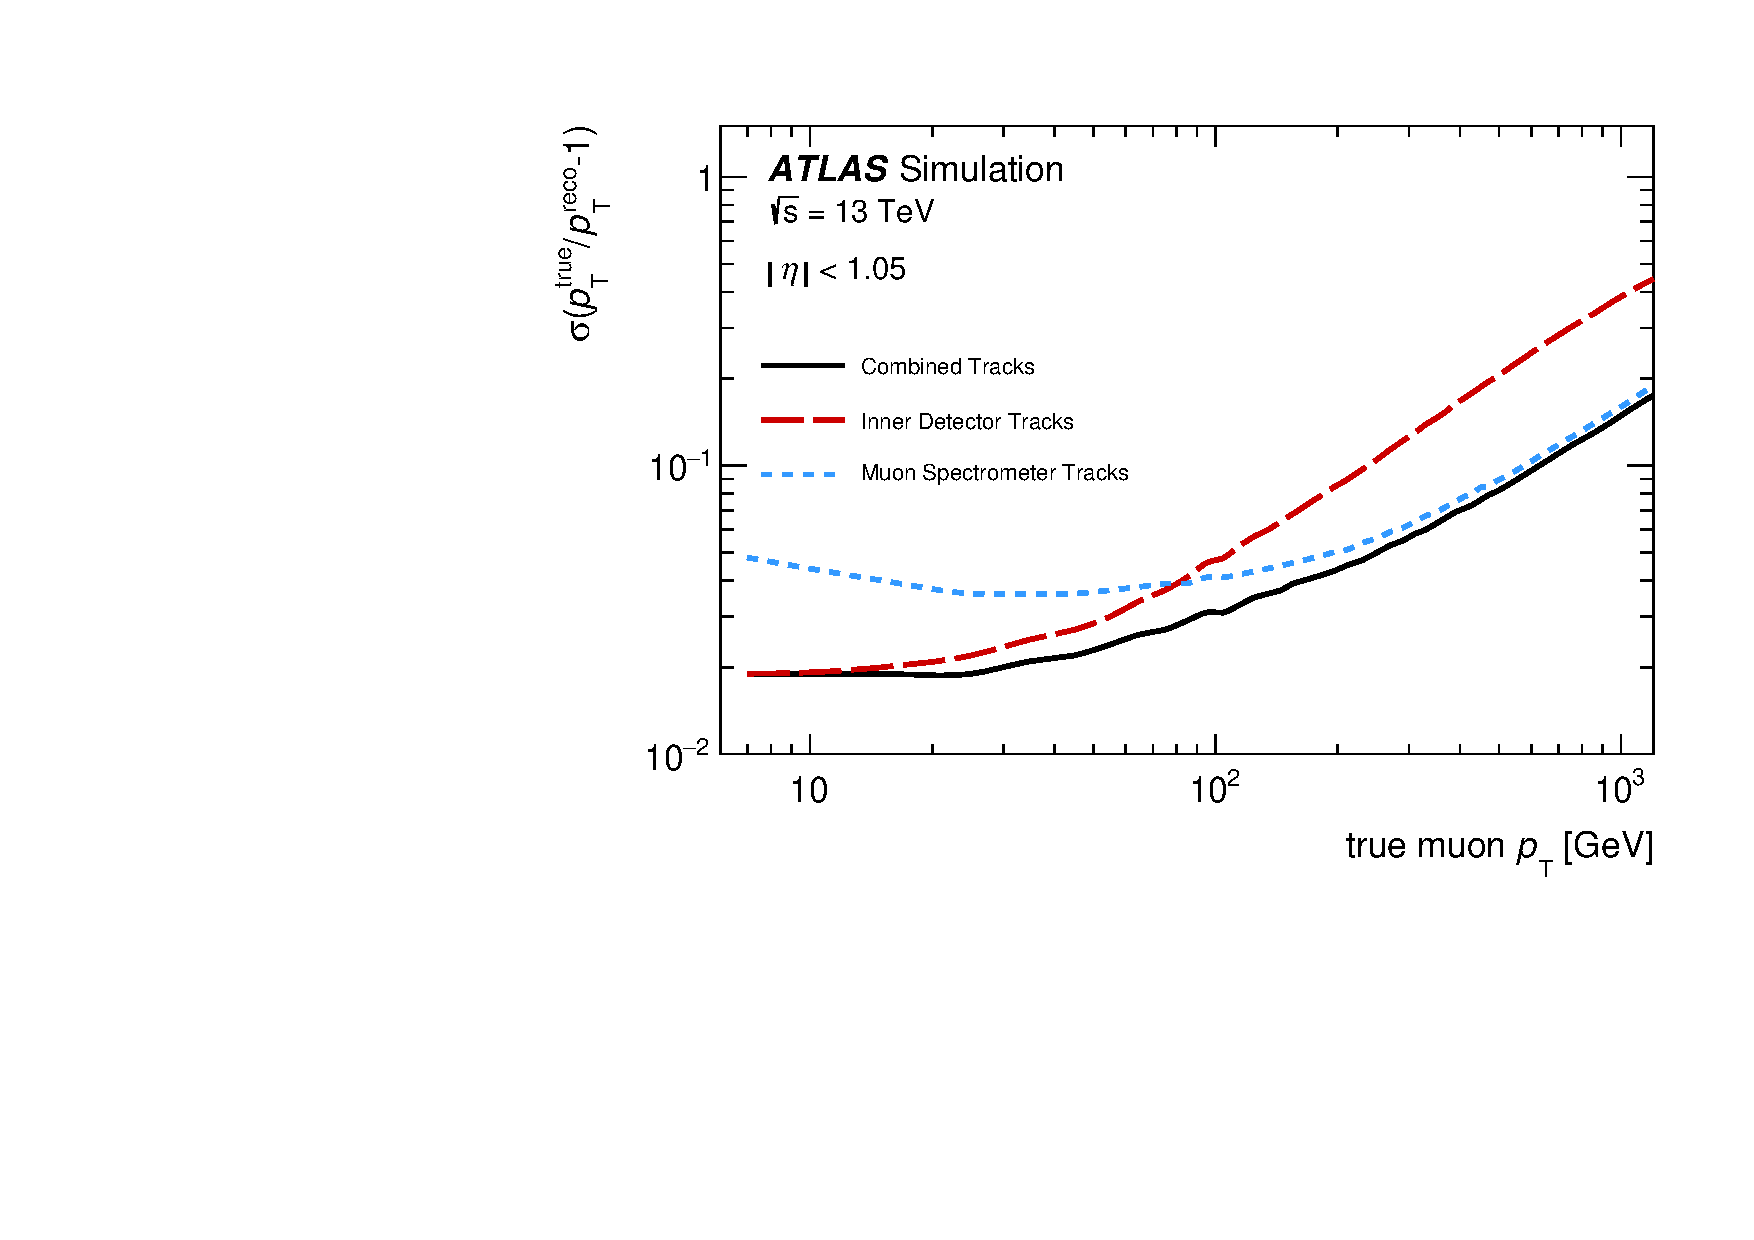
\includegraphics[width=0.495\textwidth]{muon_reco_reso_loeta.pdf}
            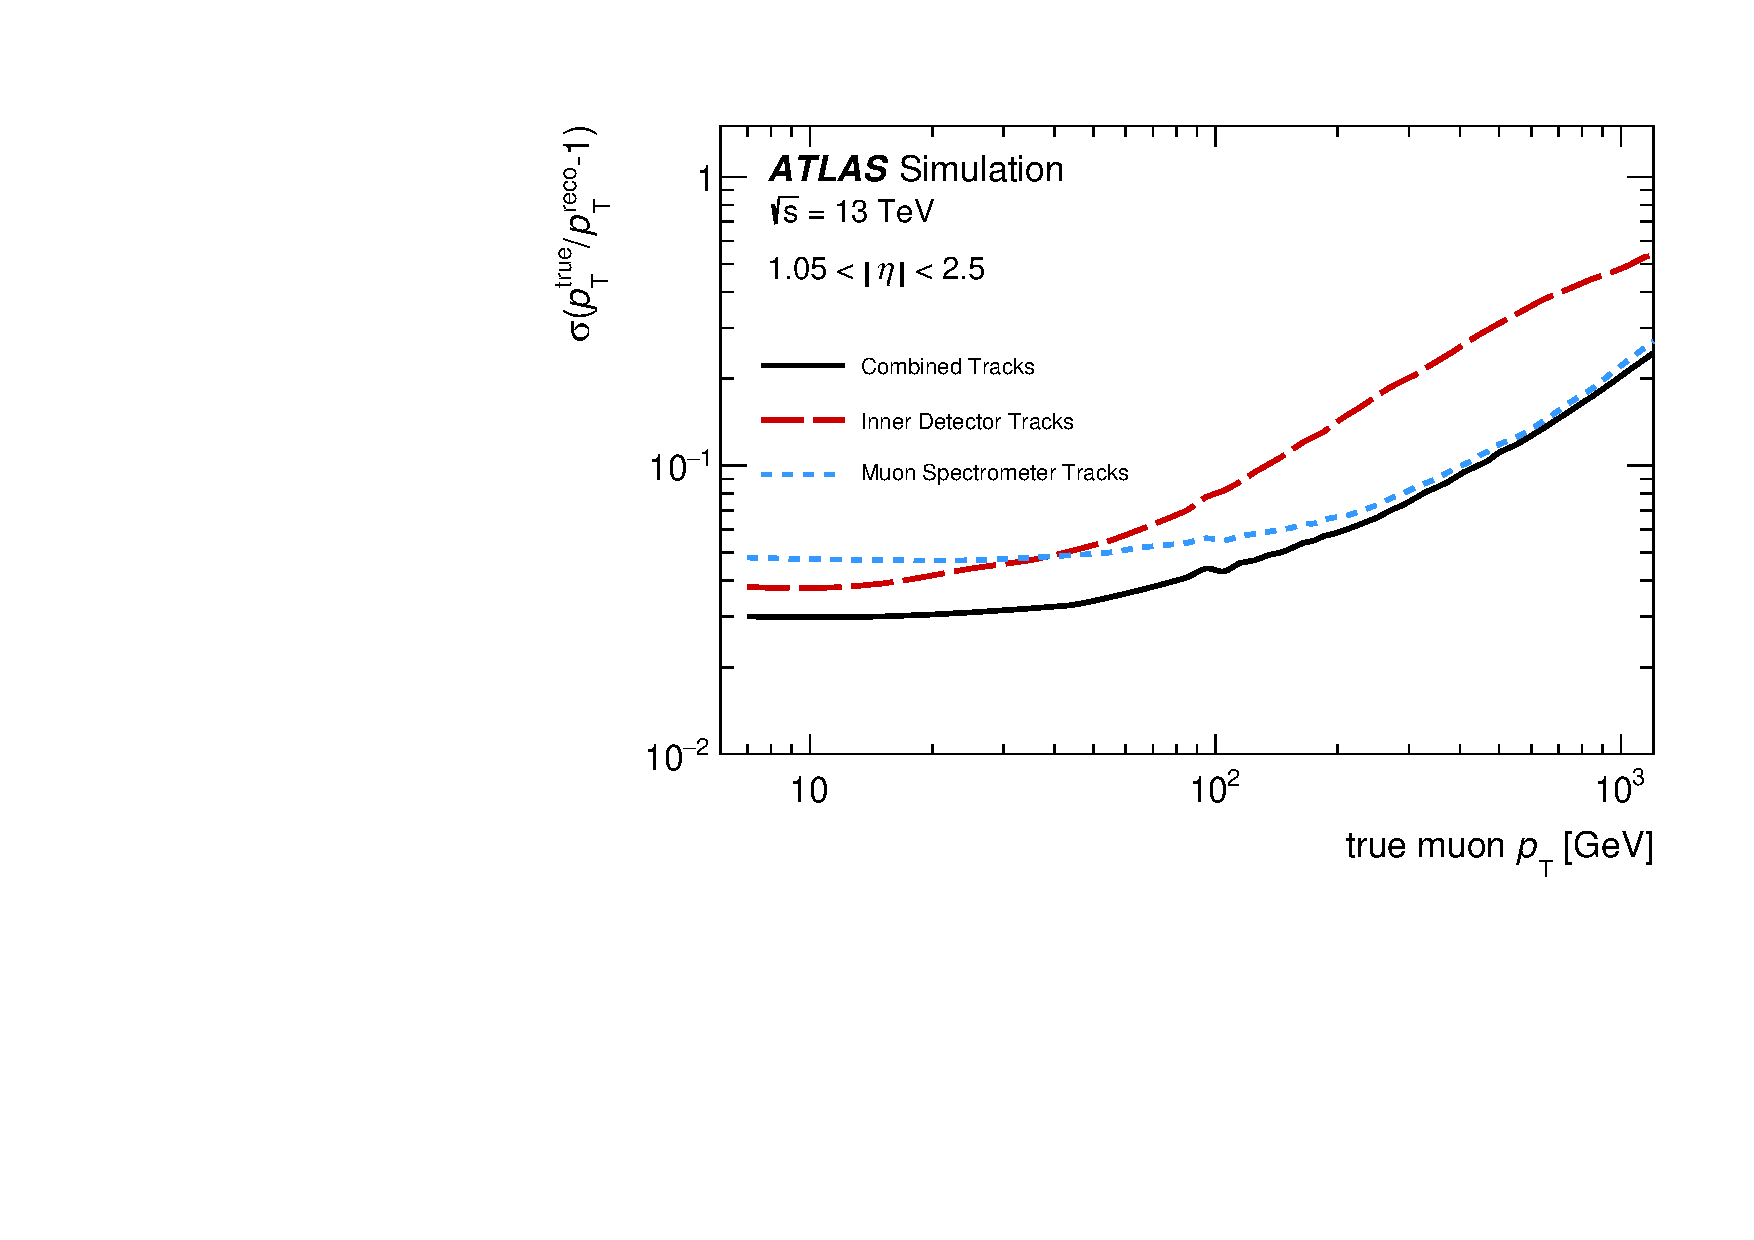
\includegraphics[width=0.495\textwidth]{muon_reco_reso_hieta.pdf}
            \caption{
                Resolution of the muon $\pt$ as obtained from simulation after derivation and application of all correction constants. 
                Muons are selected using the High-$\pt$ Working point. 
                The resolution is shown as a function of the true $\pt$ of the muon for a range from 1 GeV to 2.5 TeV, 
                (left) for muons with $|\eta|<1.05$ and (right) for muons with $|\eta|>1.05$. 
                The resolution lines are obtained by interpolating between points sampled in steps of $\pt$. 
                The continuous lines correspond to the combined momentum, while the dashed lines to that from the ID, and the dotted lines to that of the MS.
                These figures are taken from~\cite{MUON-2022-01}.
            }
            \label{fig:muon_reso}
        \end{figure}
    
    \subsection{Forward Detector}
        The forward detector systems of the ATLAS experiment~\cite{ATLAS-TDR-18} play crucial roles in measuring luminosity, 
        studying diffractive events, and characterising the centrality of heavy-ion collisions. These 
        detectors extend the capabilities of ATLAS by covering the forward regions, providing essential 
        data that complement the central detector systems. Figure \ref{fig:Forward_detectors} shows the
        layout of the forward detectors in the ATLAS experiment.
        \begin{figure}[htbp]
            \centering
            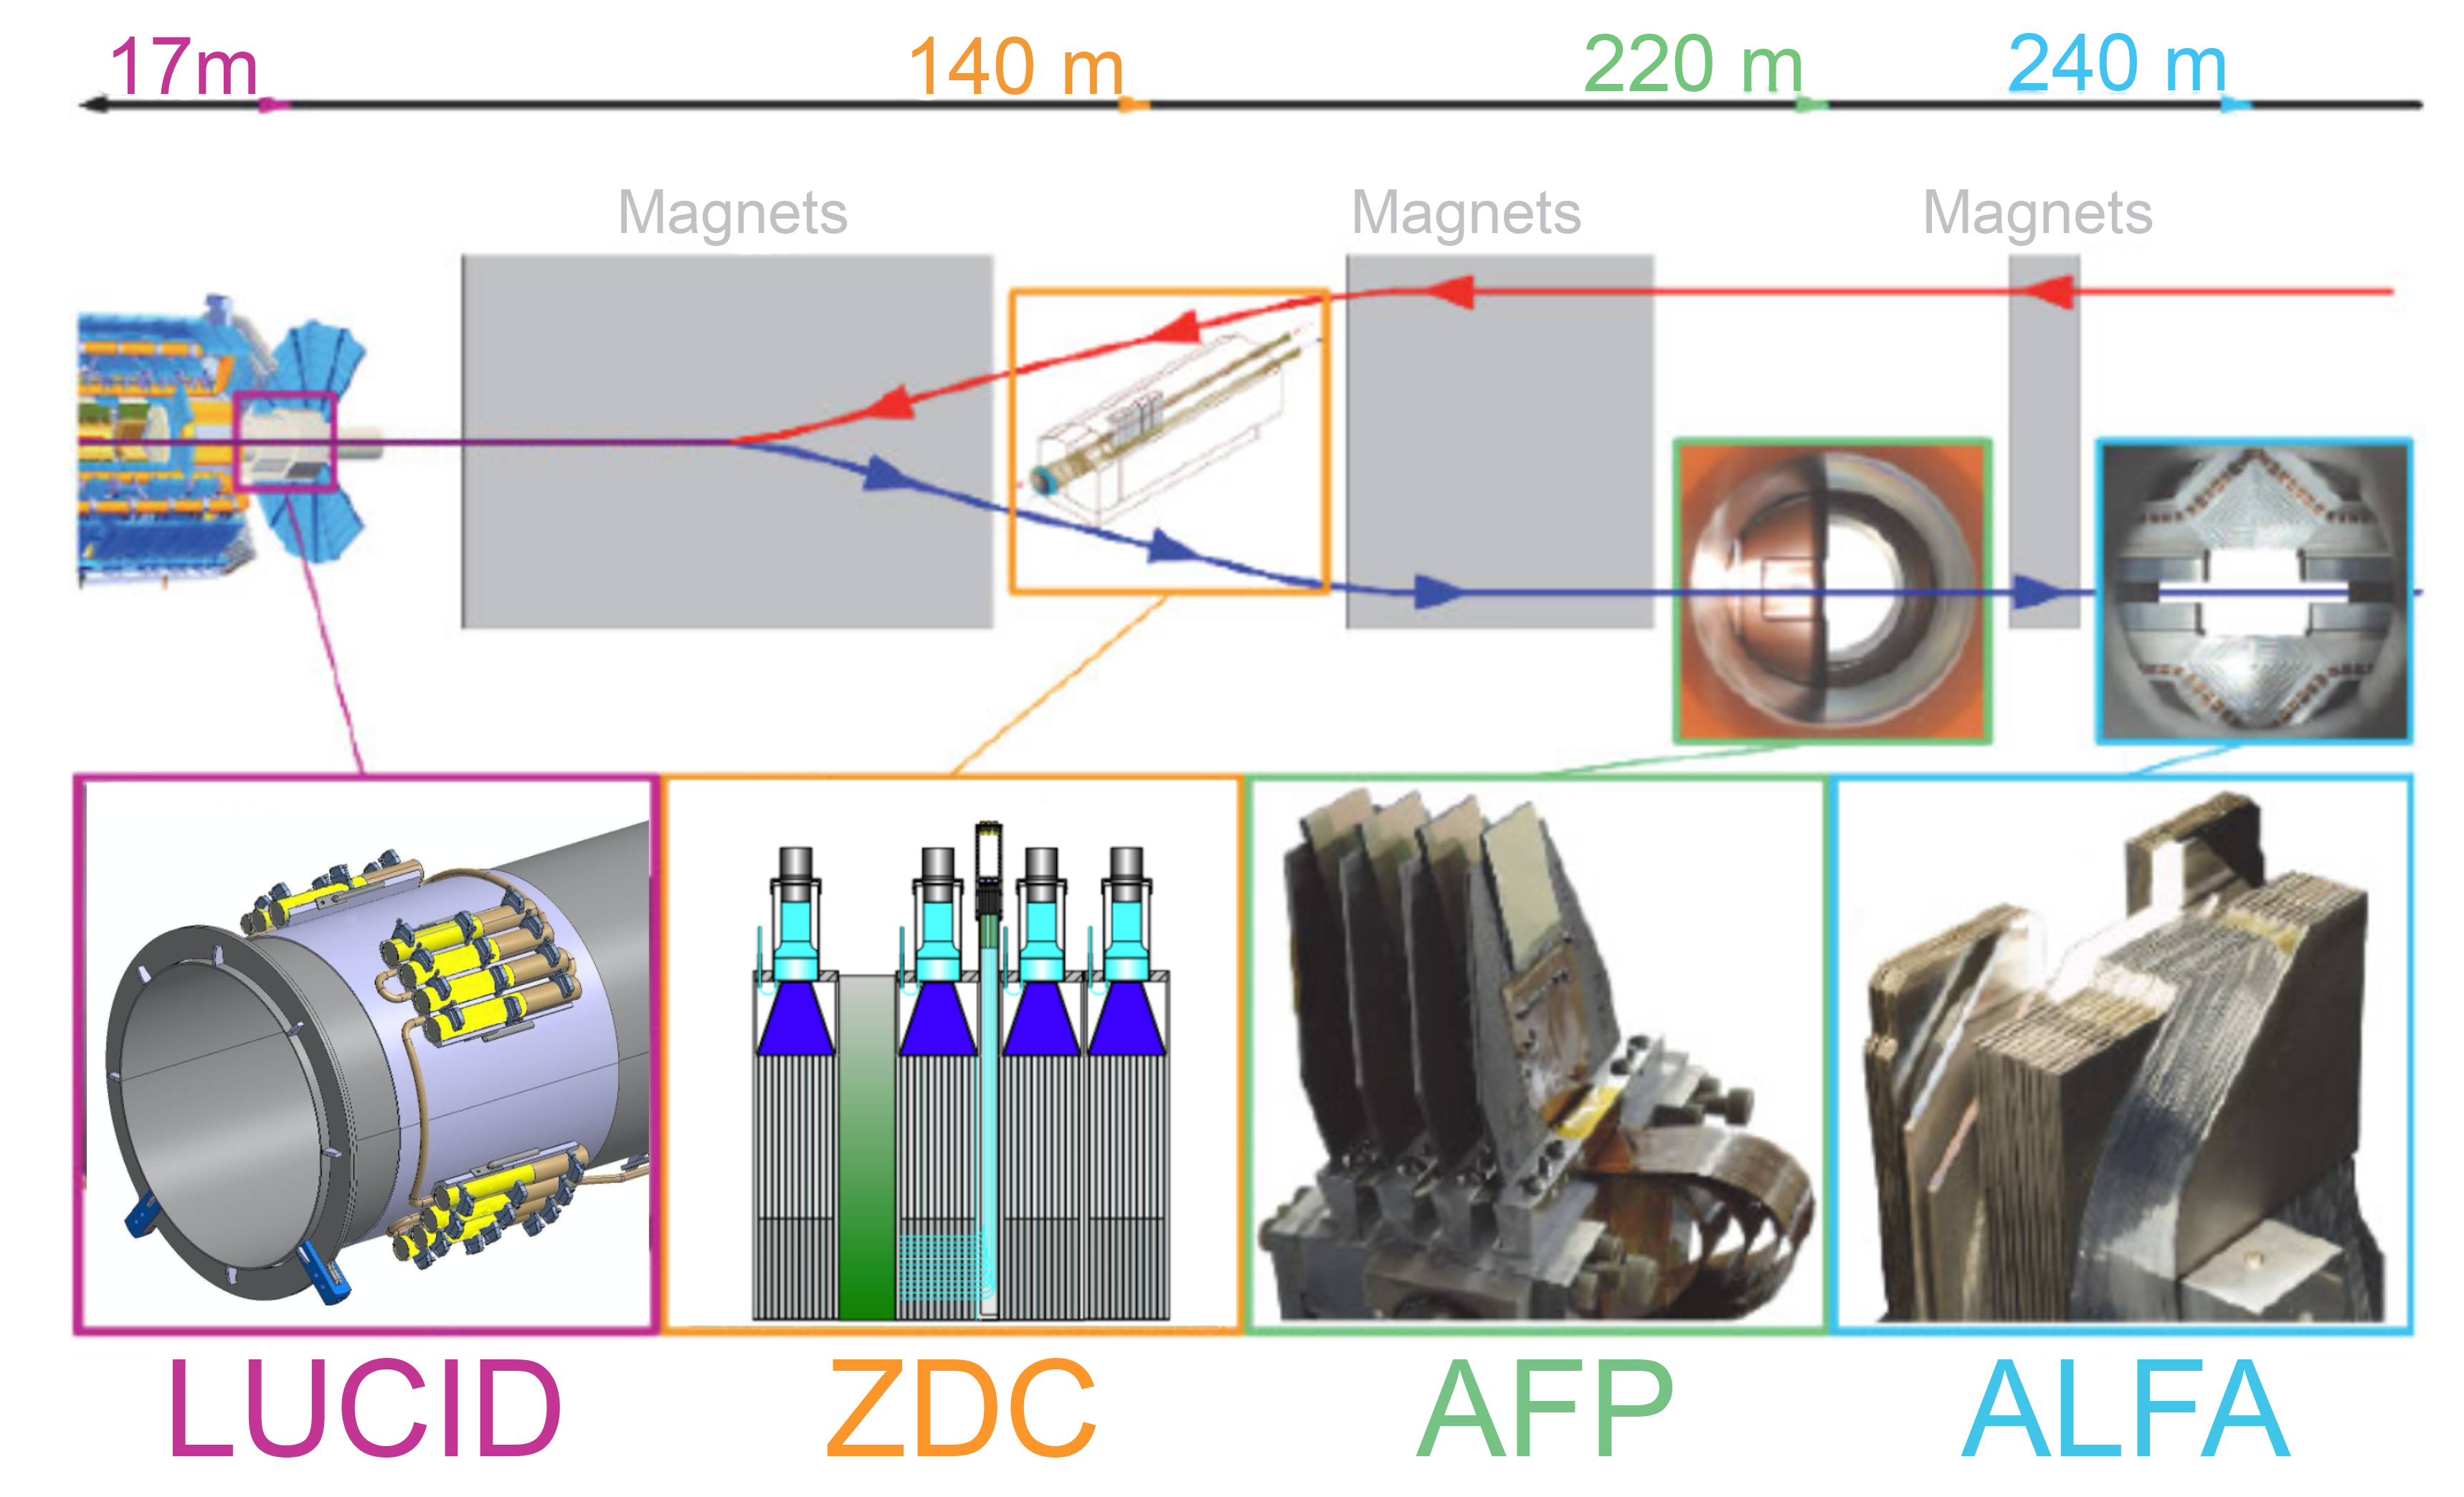
\includegraphics[width=1.0\textwidth]{ATLAS-FD-run3.png}
            \caption{Layout of the forward detectors in the ATLAS experiment, taken from~\cite{GENR-2019-02}.}
            \label{fig:Forward_detectors}
        \end{figure}

        The LUminosity Cherenkov Integrating Detector (LUCID)~\cite{LUCID2} is located at a distance of $\pm17$ meters 
        from the IP. It is primarily designed to monitor the luminosity online and offline by detecting 
        inelastic proton-proton scattering events in the forward direction. LUCID employs Cherenkov tubes 
        filled with $C_4F_{10}$ gas, which emit light when traversed by charged particles produced in 
        collisions. This light is then detected by photomultiplier tubes (PMTs), allowing for precise 
        luminosity measurements.

        The Zero Degree Calorimeters (ZDC) are located at $\pm140$ meters from the IP, just beyond where 
        the common straight-section vacuum pipe splits into two separate beampipes. The ZDC modules 
        consist of alternating layers of tungsten plates and quartz rods, optimised for detecting neutral 
        particles at pseudorapidities \(|\eta| \geq 8.2\). The ZDCs play a crucial role in determining the 
        centrality of heavy-ion collisions, providing insights into the collision geometry and the energy 
        deposition of forward-going neutrons and photons.

        The Absolute Luminosity for ATLAS (ALFA) Roman Pot detector consists of four stations positioned at $\pm240$
        meters from the IP. Each station includes two scintillating fibre trackers housed in Roman pots, 
        which can approach the LHC beam as close as 1 mm. ALFA is used in dedicated low-luminosity and 
        high-\(\beta^*\) runs to measure the total cross-section for proton-proton interactions through 
        elastic scattering and diffraction studies. In preparation of Run 3, 
        several upgrades were made to ALFA. The aged readout electronics and scintillating
        fibres were replaced, and additional shielding walls were installed to reduce radiation exposure
        and extend the operational lifespan of the detectors. The Roman Pot movement system was refurbished,
        and firmware updates were implemented for the central trigger processor input module to enhance 
        trigger and readout capabilities for ALFA-specific runs.

        The ATLAS Forward Proton (AFP) detector, part of the Phase I upgrade, is situated at $\pm205$ meters 
        (near stations) and $\pm217$ meters (far stations) from the IP. Each station contains a silicon 
        tracker (SiT) similar to the Insertable B-Layer (IBL) and a Time-of-Flight (ToF) detector. The 
        SiT provides precise measurements of the proton trajectories, while the ToF detector measures 
        the time difference between protons reaching the detectors, achieving vertex resolution of 3 to 5 mm.

        The AFP detector underwent several upgrades during LS2 to prepare for Run 3. These upgrades included:
        \begin{itemize}
            \item replacement of radiation-damaged silicon detectors with new 3D silicon pixel tracker modules.
            \item redesign of the ToF detector to prevent corona discharge issues in vacuum.
            \item updates to the trigger and readout electronics to improve timing resolution and data acquisition efficiency.
        \end{itemize}

        \begin{figure}[htbp]
            \centering
            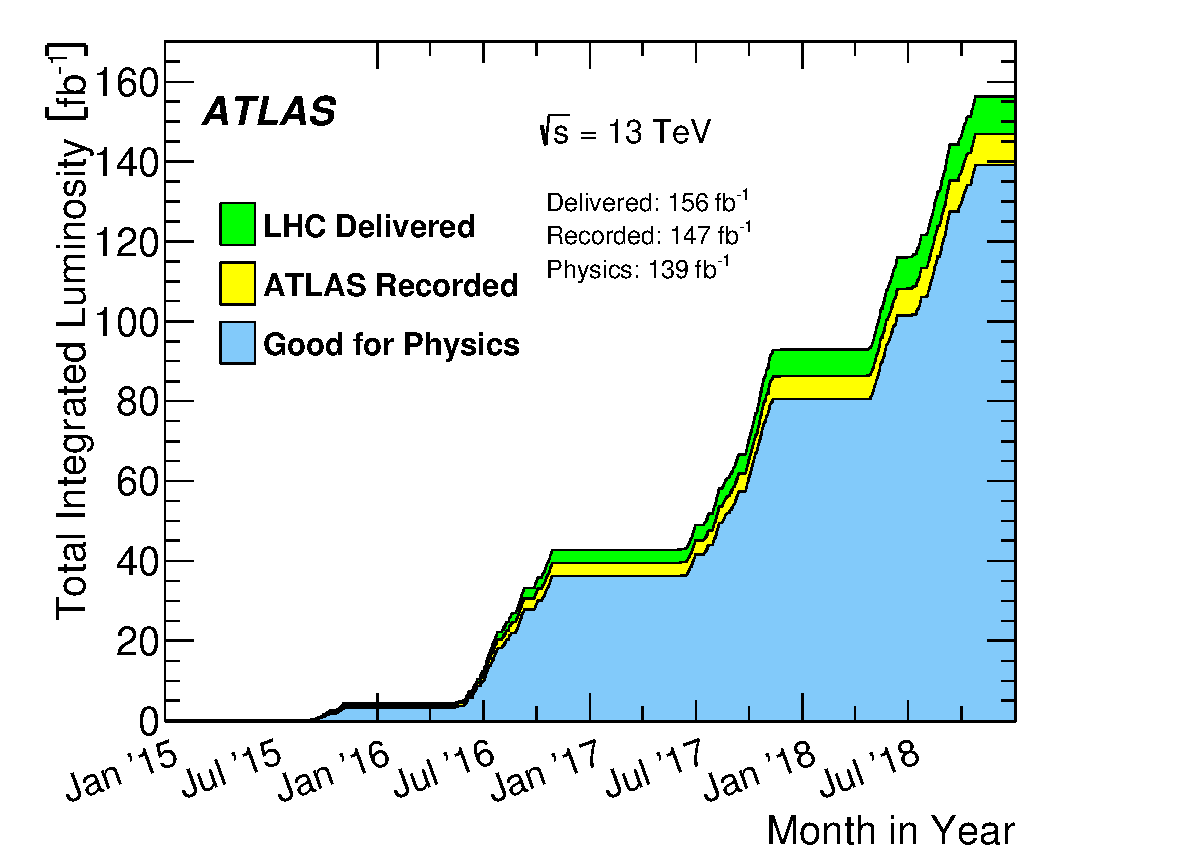
\includegraphics[width=0.5\textwidth]{total_lumi_run2.pdf}
            \caption{
                Cumulative integrated luminosity delivered to and recorded by ATLAS between 2015 and 2018 during stable beam pp collision data-taking at $\sqrt{s}=13$ TeV. This figure is taken from~\cite{DAPR-2018-01}.
            }
            \label{fig:run2lumi}
        \end{figure}

    \subsection{TDAQ System}
        The Trigger and Data Acquisition (TDAQ)~\cite{ATLAS-TDR-16} system of the ATLAS detector is a 
        sophisticated infrastructure designed to manage the immense amount of data generated by particle 
        collisions at the LHC. Its primary function is to select and record the most interesting 
        collision events for detailed analysis, thereby enabling the identification of rare physics 
        phenomena. A schematic of the ATLAS TDAQ system is shown in Figure~\ref{fig:TDAQ_schematic}.
        \begin{figure}[htbp]
            \centering
            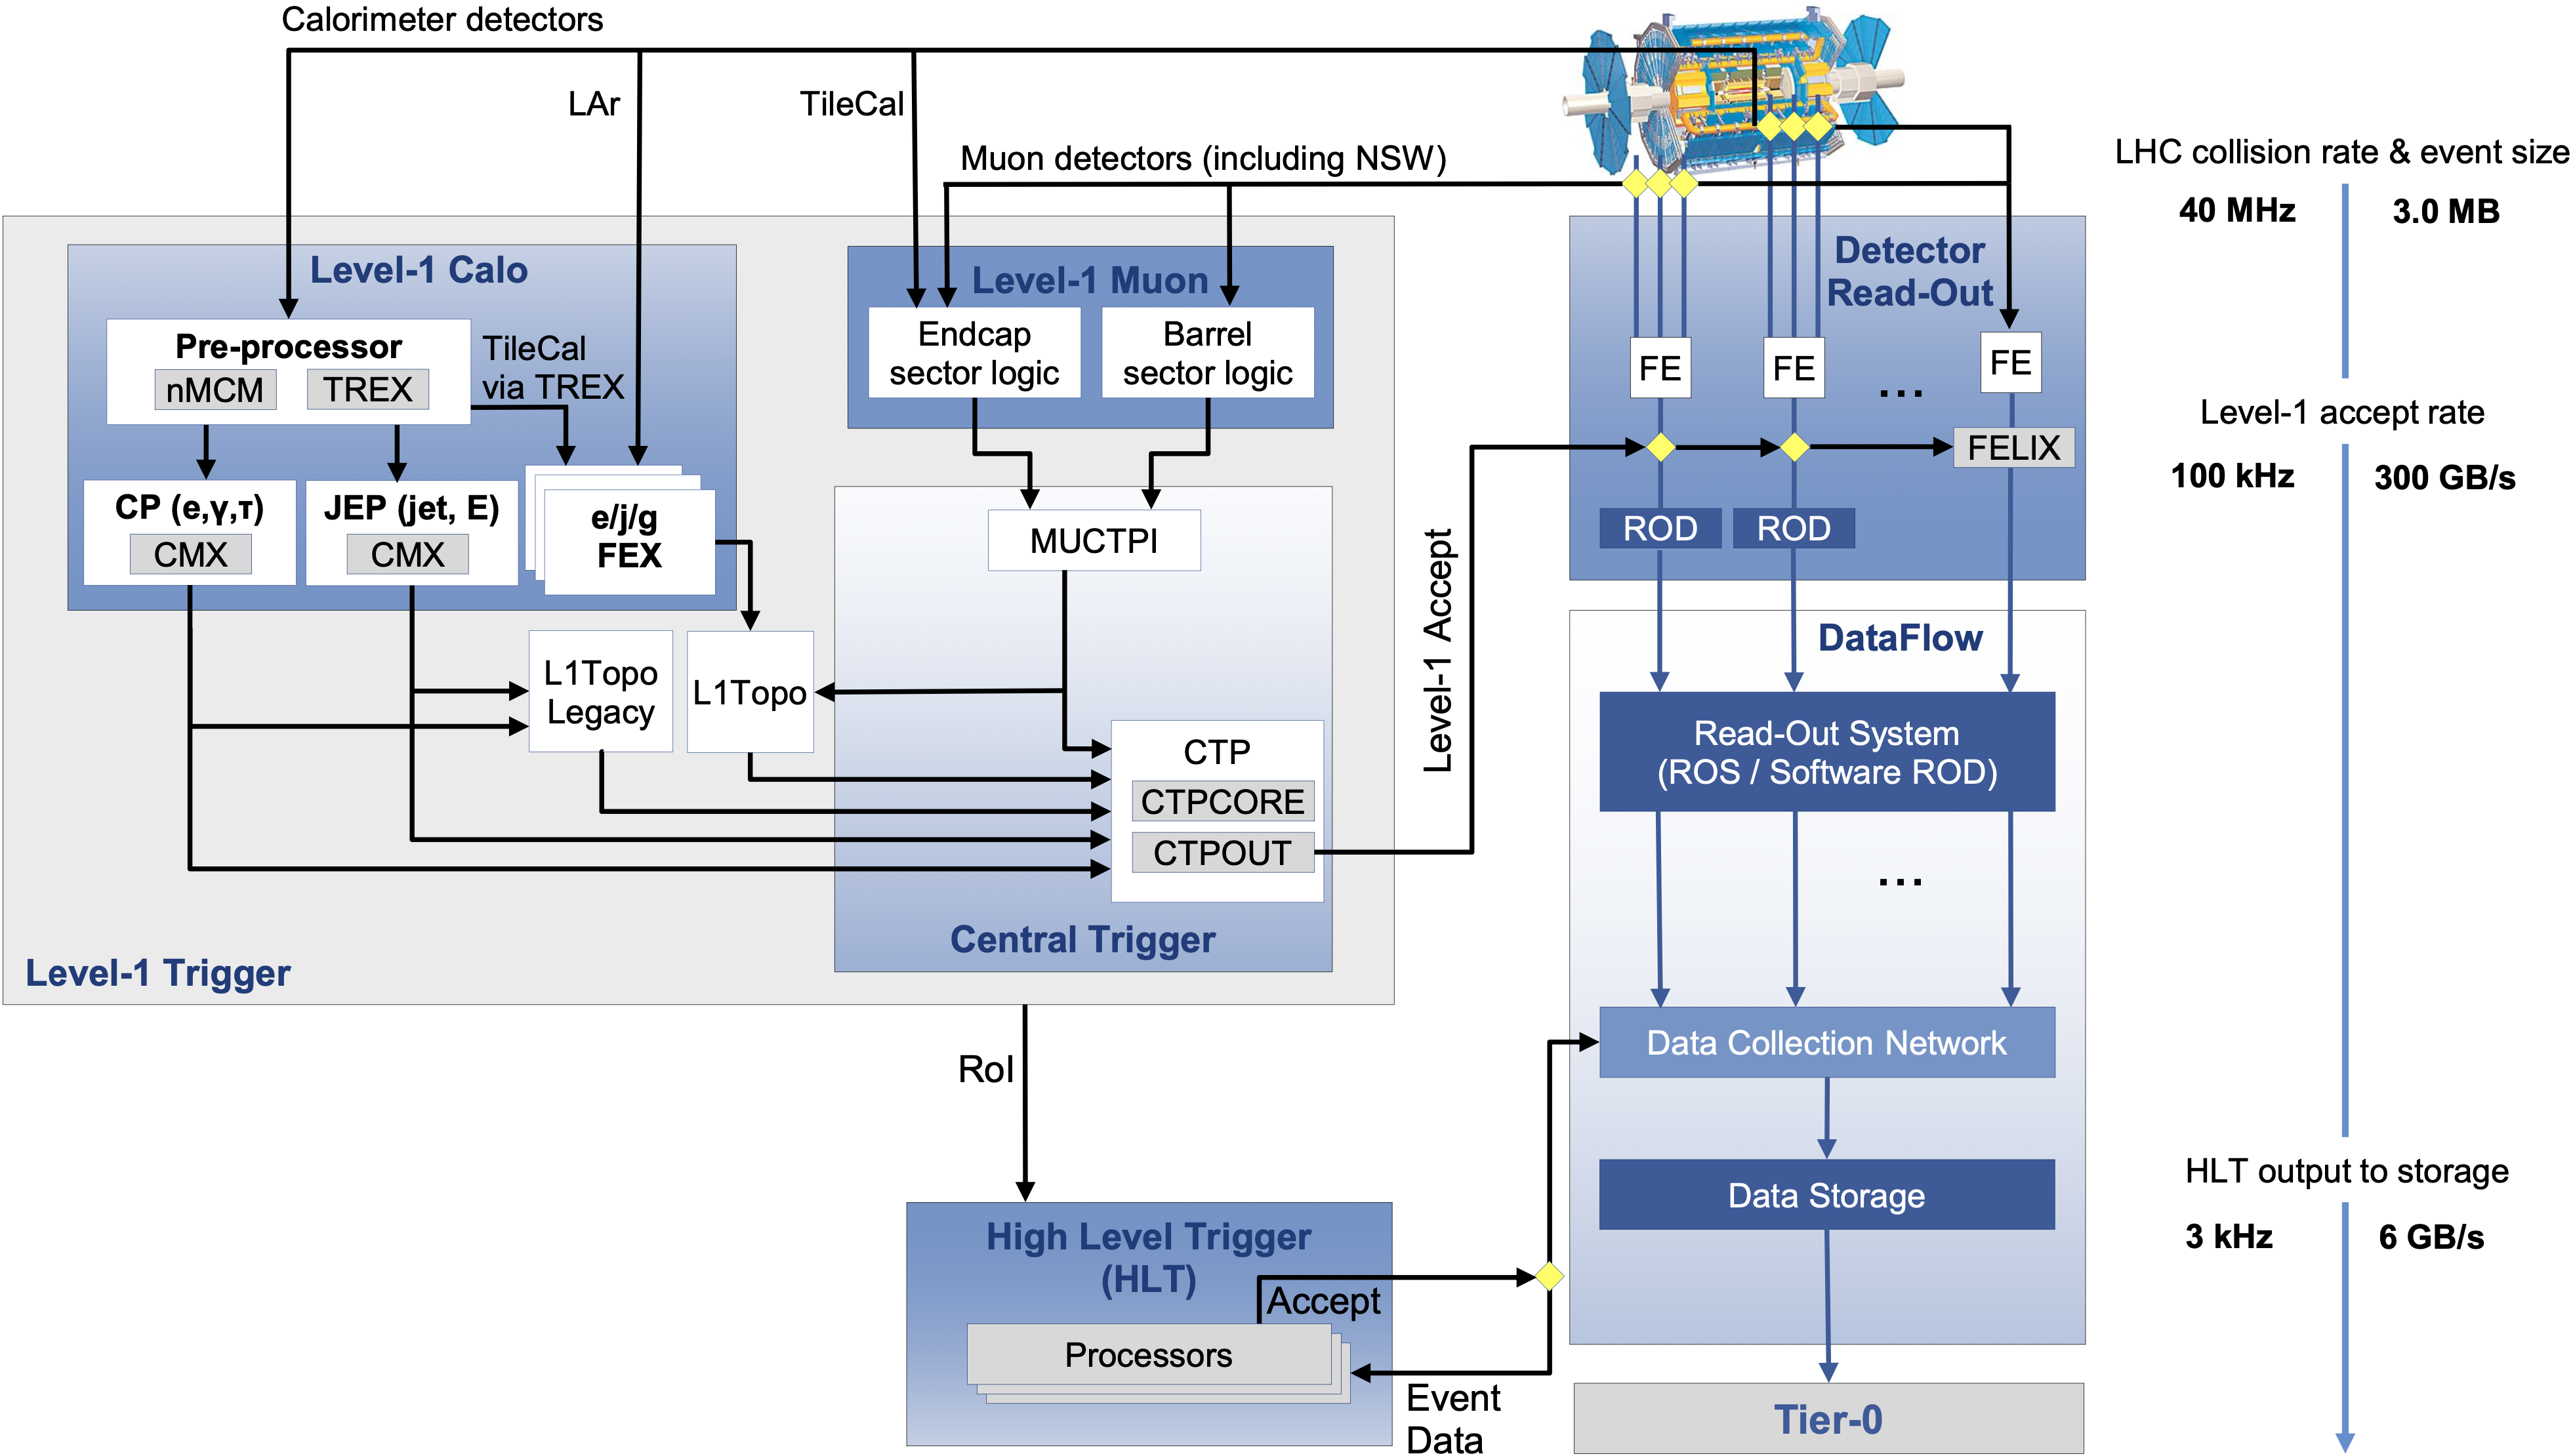
\includegraphics[width=1.0\textwidth]{ATLAS-TDAQ-run3.png}
            \caption{Schematic of the ATLAS Trigger and Data Acquisition (TDAQ) system, taken from~\cite{GENR-2019-02}.}
            \label{fig:TDAQ_schematic}
        \end{figure}
        The ATLAS TDAQ system employs a multi-tiered architecture that comprises the Level-1 (L1) Trigger, 
        the High-Level Trigger (HLT), and the Data Acquisition (DAQ) system. This design allows for efficient 
        and rapid data processing, ensuring that only the most relevant events are stored for further analysis. 

        The L1 Trigger is the first stage in the event-selection process. It operates directly on the raw data 
        from the detector, using custom-built hardware to analyse data with reduced granularity. The L1 Trigger 
        must make decisions within a strict latency of 2.5 microseconds to reduce the event rate from the 40 MHz 
        bunch crossing rate of the LHC to a maximum of 100 kHz. The L1 Trigger comprises the L1 calorimeter 
        triggers and the L1 muon triggers. Both subsystems generate Region of Interest (RoI) signals that guide 
        the HLT in its more detailed analysis.
        The HLT is a software-based system implemented on commercial processors. It performs detailed event 
        reconstruction using the full detector data, significantly refining the initial L1 selection. 
        The HLT reduces the event rate from the L1's 100 kHz to about 3 kHz for storage. Guided by RoIs from 
        the L1 Trigger, the HLT performs localised and full-event reconstruction. For Run 3, the HLT uses the 
        AthenaMT software framework, which allows for parallel processing and more efficient resource use. 
        Sophisticated algorithms, including those for track reconstruction and particle identification, 
        enhance the precision and efficiency of event-selection.
        The DAQ system is responsible for managing data flow from the detector front-end electronics to permanent 
        storage. It ensures that data from accepted events are properly formatted, transported, and recorded.
        Key components of the DAQ system include:
        \begin{itemize}
            \item Readout System (ROS): The ROS collects data from sub-detectors following an L1 accept and 
            buffers it for HLT processing.
            \item Data Collection Network: This high-bandwidth network facilitates data transfer from the 
            ROS to the HLT processing farm.
            \item Data Storage: Events accepted by the HLT are transferred to permanent storage for offline 
            analysis. The system is designed to handle an average output of 3 kHz, corresponding to a data 
            throughput of 6 GB/s.
        \end{itemize}
        Several upgrades have been implemented in the TDAQ system for Run 3~\cite{ATLAS-TDR-23} to cope with higher luminosities 
        and increased data rates. Upgraded L1 Trigger electronics and algorithms provide finer granularity 
        and improved selectivity, allowing for better background rejection and more efficient event-selection.
        Level-2 (L2) and event filter (EF) systems used in the previous runs have been integrated into a 
        single HLT framework, streamlining the data processing pipeline and improving resource utilisation.
        The computational resources of the TDAQ systems have been expanded to handle the increased data 
        volume and complexity, ensuring that event reconstruction and selection can be performed with high 
        efficiency. Enhancements in data management and storage infrastructure ensure that the system can 
        handle the increased data volume and maintain data integrity.
\section{Object reconstruction and identification in ATLAS} 
    \subsection{Reconstruction and identification of electrons and photons} 
        \subsubsection{Egamma reconstruction}
            The reconstruction of electrons and photons (collectively known as Egamma)~\cite{EGAM-2018-01, EGAM-2021-01} in the ATLAS detector is a multi-step process that 
            involves the collection of energy deposits in the electromagnetic calorimeter and matching these deposits to tracks reconstructed 
            in the ID. The energy of electron and photon candidates is reconstructed by clustering the energy deposits in the cells of the 
            EM calorimeter. The algorithm used is optimised to handle the different shower shapes and energy distributions of electrons and 
            photons. Superclusters are formed by combining clusters from the presampler and multiple calorimeter layers, using a 
            boosted-decision-tree (BDT) regression algorithm to optimise the energy measurement. This approach accounts for variations 
            in the particle's incident angle and position within the detector. For electrons, the energy clusters are matched to tracks 
            reconstructed in the ID. The matching is based on the consistency between the cluster position and the extrapolated track position 
            at the calorimeter. A combination of criteria, including the ratio of the track momentum to the cluster energy (E/p) and the shower 
            shape, is used to enhance the identification efficiency and purity. This matching process helps distinguish electrons from hadronic 
            background and photon conversions.
            Photons are identified through their characteristic energy deposits in the EM calorimeter. Unconverted photons, which do not 
            interact in the ID, are identified purely based on the calorimeter information. Converted photons, which produce an electron-positron 
            pair in the ID, require reconstruction of the conversion vertex and matching of the resulting tracks to the calorimeter clusters. 
            The photon identification criteria involve isolation requirements and shower shape variables to reduce background from neutral hadrons and jets.
            \begin{figure}[htbp]
                \centering
                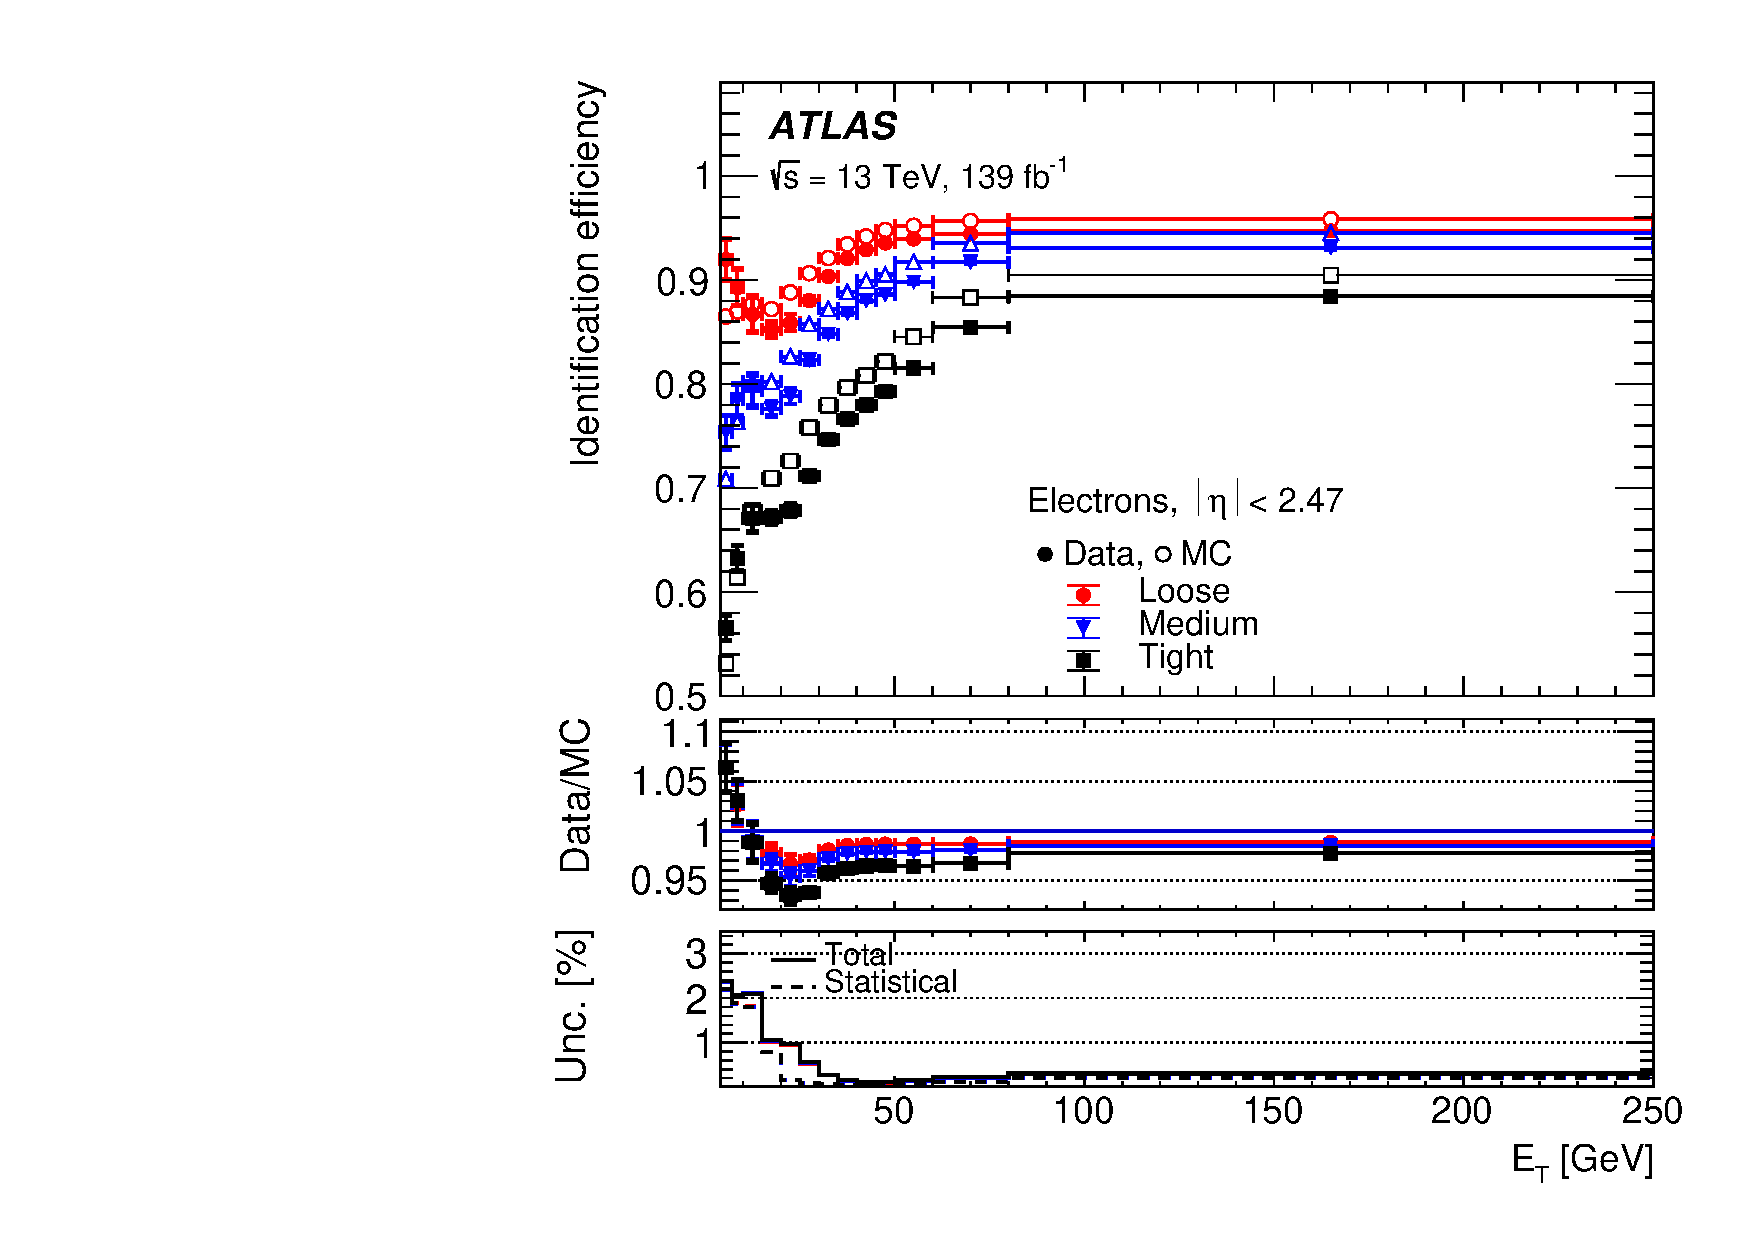
\includegraphics[width=0.5\textwidth]{elec_effi_pt.pdf}
                \caption{
                    Identification efficiencies of electrons from $Z\rightarrow ee$ decays as a function of the electron's transverse momentum for the different identification working points. This figure is taken from~\cite{EGAM-2021-01}.
                }
                \label{fig:elec_effi}
            \end{figure}
        \subsubsection{Egamma calibration}
            The calibration of electron and photon energies~\cite{EGAM-2021-02} is crucial for achieving precise measurements required for ATLAS physics analyses. 
            The calibration procedure involves several steps to correct for detector response variations and ensure consistency between data and simulation.
            The EM calorimeter is segmented into longitudinal layers, each of which responds differently to incident particles. The first step in the 
            calibration process involves correcting the energy response of each layer to account for these variations. This is achieved using detailed 
            simulations and data-driven techniques to ensure accurate energy measurements across the detector. A simulation-based BDT regression 
            algorithm is used to combine the energy deposits from different calorimeter layers and the presampler. This algorithm is trained to 
            optimise the energy measurement separately for electrons, converted photons, and unconverted photons, considering the particle's position 
            and angle of incidence. The simulation-based calibration is applied uniformly to data and simulated events. Several corrections are applied 
            to account for residual differences between data and simulation. These include adjustments for non-uniformities in the detector response, 
            variations in the high-voltage settings, and corrections for biases introduced by the liquid-argon calorimeter electronics. The stability 
            of the calorimeter response over time and across different detector regions is also monitored and corrected as necessary. The final calibration 
            step involves adjusting the global energy scale using samples of $Z \rightarrow ee$ events. The peak of the reconstructed Z boson mass is 
            aligned between data and simulation to ensure consistency. This step also includes smearing the energy resolution in the simulation to match 
            that observed in the data, thereby correcting for any discrepancies in the detector's energy response. Photon-specific calibration steps are 
            needed to account for differences in the lateral development of electron and photon showers. Corrections are derived from studies of out-of-cluster 
            energy leakage and the modelling of photon reconstruction efficiencies. These corrections ensure that the energy measurements for photons are 
            as precise as those for electrons.

            The calibrated energy measurements are validated using independent data samples, such as $J/\psi \rightarrow ee$ and $Z \rightarrow ll\gamma$ events. 
            The systematic uncertainties associated with the calibration are thoroughly evaluated, accounting for factors such as the passive material model, 
            the electronic noise, and the pile-up conditions. 

        \subsubsection{Neural Network (NN) based electron identification}
            Two significant developments in this area are the use of Deep Neural Networks (DNNs)~\cite{ATL-PHYS-PUB-2022-022} and Convolutional Neural Networks (CNNs)~\cite{ATL-DAPR-PUB-2023-001}
            for electron identification.
            The DNN-based electron identification algorithm leverages high-level discriminating variables derived from the reconstructed electron track and calorimeter 
            energy deposits. The DNN algorithm enhances electron identification performance by optimising the correlations between input features, which are often 
            neglected in traditional likelihood-based approaches. By performing multinomial classification, the DNN can categorise electron backgrounds into several 
            classes, such as electrons from heavy-flavour decays or light-flavour hadrons, enabling targeted background rejection. This approach has demonstrated 
            a significant increase in combined background rejection, with improvements ranging from 1.7 to 5.5 times compared to previous methods for a fixed signal efficiency.
            The CNN-based algorithm further refines electron identification by processing low-level detector information, such as calorimeter cell energy deposits, 
            which are treated as images. The CNN architecture is specialised in image recognition, allowing it to effectively analyse the spatial patterns of energy 
            deposits. This algorithm integrates high-level features used in DNNs and additional tracks matched to electron candidates, which enhances its performance. 
            The CNN has shown remarkable improvements in background rejection, particularly for light-flavour hadrons and electrons from photon conversions. For 
            instance, it achieves background rejection factors up to five times better than the likelihood-based method for charged hadrons faking electron signatures. 
            The CNN's ability to output a vector of probabilities for different electron classes further enhances its flexibility and accuracy in various analyses.

            These advancements are crucial for enhancing the precision of physics analyses conducted at the ATLAS experiment, particularly 
            those involving multiple leptons or requiring stringent electron background rejection. In the future, these neural network-based approaches will 
            continue to evolve, potentially incorporating real data for training to overcome simulation biases and improve generalisation to actual collision 
            events. Adversarial training techniques might also be employed to mitigate differences between simulated and real data, further refining the performance 
            of electron identification algorithms in ATLAS.

    \subsection{Jet reconstruction}
        Jets are collimated streams of particles that result from the hadronisation of quarks and 
        gluons produced in high-energy processes. As a direct consequence of the running of the 
        strong coupling constant, and the QCD colour confinement, when quarks and gluons are produced in a collision, 
        they cannot exist freely. Instead, they fragment into a cascade of hadrons, predominantly 
        pions and kaons, which cluster together to form jets. The ATLAS experiment employs sophisticated 
        jet reconstruction techniques to accurately identify and measure jets. 
        The reconstruction processes have evolved to utilise both calorimetric and tracking information, 
        enhancing the precision and robustness of jet measurements. The two primary methods are based on calorimeter 
        information and the particle flow (PFlow) algorithm~\cite{PERF-2015-09}, both of which use the anti-kt 
        algorithm~\cite{Cacciari:2008gp} with a radius parameter \( R = 0.4 \). A larger radius parameter 
        (\( R = 1.0 \)) is used for large-radius jets optimised for boosted object identification~\cite{JETM-2023-02}.

        \subsubsection{Calorimeter-based jet reconstruction}
            In the calorimeter-based method, jets are reconstructed using three-dimensional topological clusters 
            (topo-clusters)~\cite{PERF-2014-07, JETM-2023-01} of calorimeter cells. These cells are grouped together based on their energy depositions 
            and spatial proximity using a nearest-neighbour algorithm. The energy of these clusters is initially 
            calibrated to the electromagnetic (EM) energy scale, which is suitable for measuring energy depositions from 
            electromagnetic showers. Only positive-energy topo-clusters are used as inputs to the jet reconstruction. 
            An origin correction is applied to each topo-cluster to account for the position of the primary vertex, 
            ensuring that the jet's energy and direction are accurately determined with respect to the event's primary vertex.

            EMtopo jets, reconstructed using origin-corrected EM scale topo-clusters, 
            were the primary jet definition used in ATLAS physics analyses conducted in Run 2. 
            These jets exhibited robust energy scale and resolution characteristics 
            across a wide kinematic range and were independent of other reconstruction algorithms such as tracking at the 
            jet-building stage~\cite{JETM-2018-05}.

        \subsubsection{Particle Flow (PFlow) algorithm}
            The particle flow algorithm aims to improve jet reconstruction by combining measurements from both 
            the tracking and calorimeter systems~\cite{JETM-2018-05}. This approach reconstructs individual particles by replacing 
            the energy deposited in the calorimeter by charged particles with the momenta of tracks matched to 
            those deposits. The PFlow algorithm uses the following steps:
            \begin{itemize}
                \item Track Selection: Tracks are selected based on quality criteria, such as a transverse momentum 
                (\( p_T \)) threshold of 500 MeV and a distance of closest approach to the primary vertex along the 
                z-axis less than 2 mm. This selection helps to suppress pile-up contributions by rejecting tracks not 
                associated with the primary vertex.
                \item Energy Subtraction: The energy deposited by charged particles in the calorimeter is subtracted, 
                and the corresponding track momenta are used instead. This subtraction is carefully managed to avoid 
                removing energy deposited by other particles.
                \item Topo-Cluster Adjustment: The \( \eta \) and \( \phi \) coordinates of topo-clusters are recomputed
                with respect to the primary vertex position. This adjustment ensures that the reconstructed jets are aligned 
                correctly with the hard-scatter interaction.
            \end{itemize}
            PFlow jets, formed from these combined signals, exhibit improved energy and angular resolution, reconstruction 
            efficiency, and stability against pile-up effects compared to jets reconstructed using calorimeter information alone.

        \subsubsection{Jet calibration and performance}
            Calibration of the reconstructed jets involves several steps to ensure their energy scale matches the particle level~\cite{JETM-2018-05, JETM-2022-01}. 
            Firstly, pile-up corrections remove excess energy due to additional proton-proton interactions within the same or nearby 
            bunch crossings. They consist of a jet area-based correction and a residual correction derived from Monte Carlo (MC) simulations.
            The second step is the absolute energy scale calibration, this step corrects the jet energy and direction to match those of 
            particle-level truth jets. It is typically derived from dijet MC events. Then, the global sequential calibration process 
            reduces the dependence of the reconstructed jet response on tracking, calorimeter, and muon chamber information, further 
            refining the energy resolution and reducing systematic uncertainties. Finally, the in situ calibration corrects any remaining
            differences between data and MC simulation using well-measured reference objects such as photons, Z bosons, and calibrated jets.
            The final step is applied to data only.
            These methods ensure that ATLAS can precisely reconstruct and measure jets.
            \begin{figure}[htbp]
                \centering
                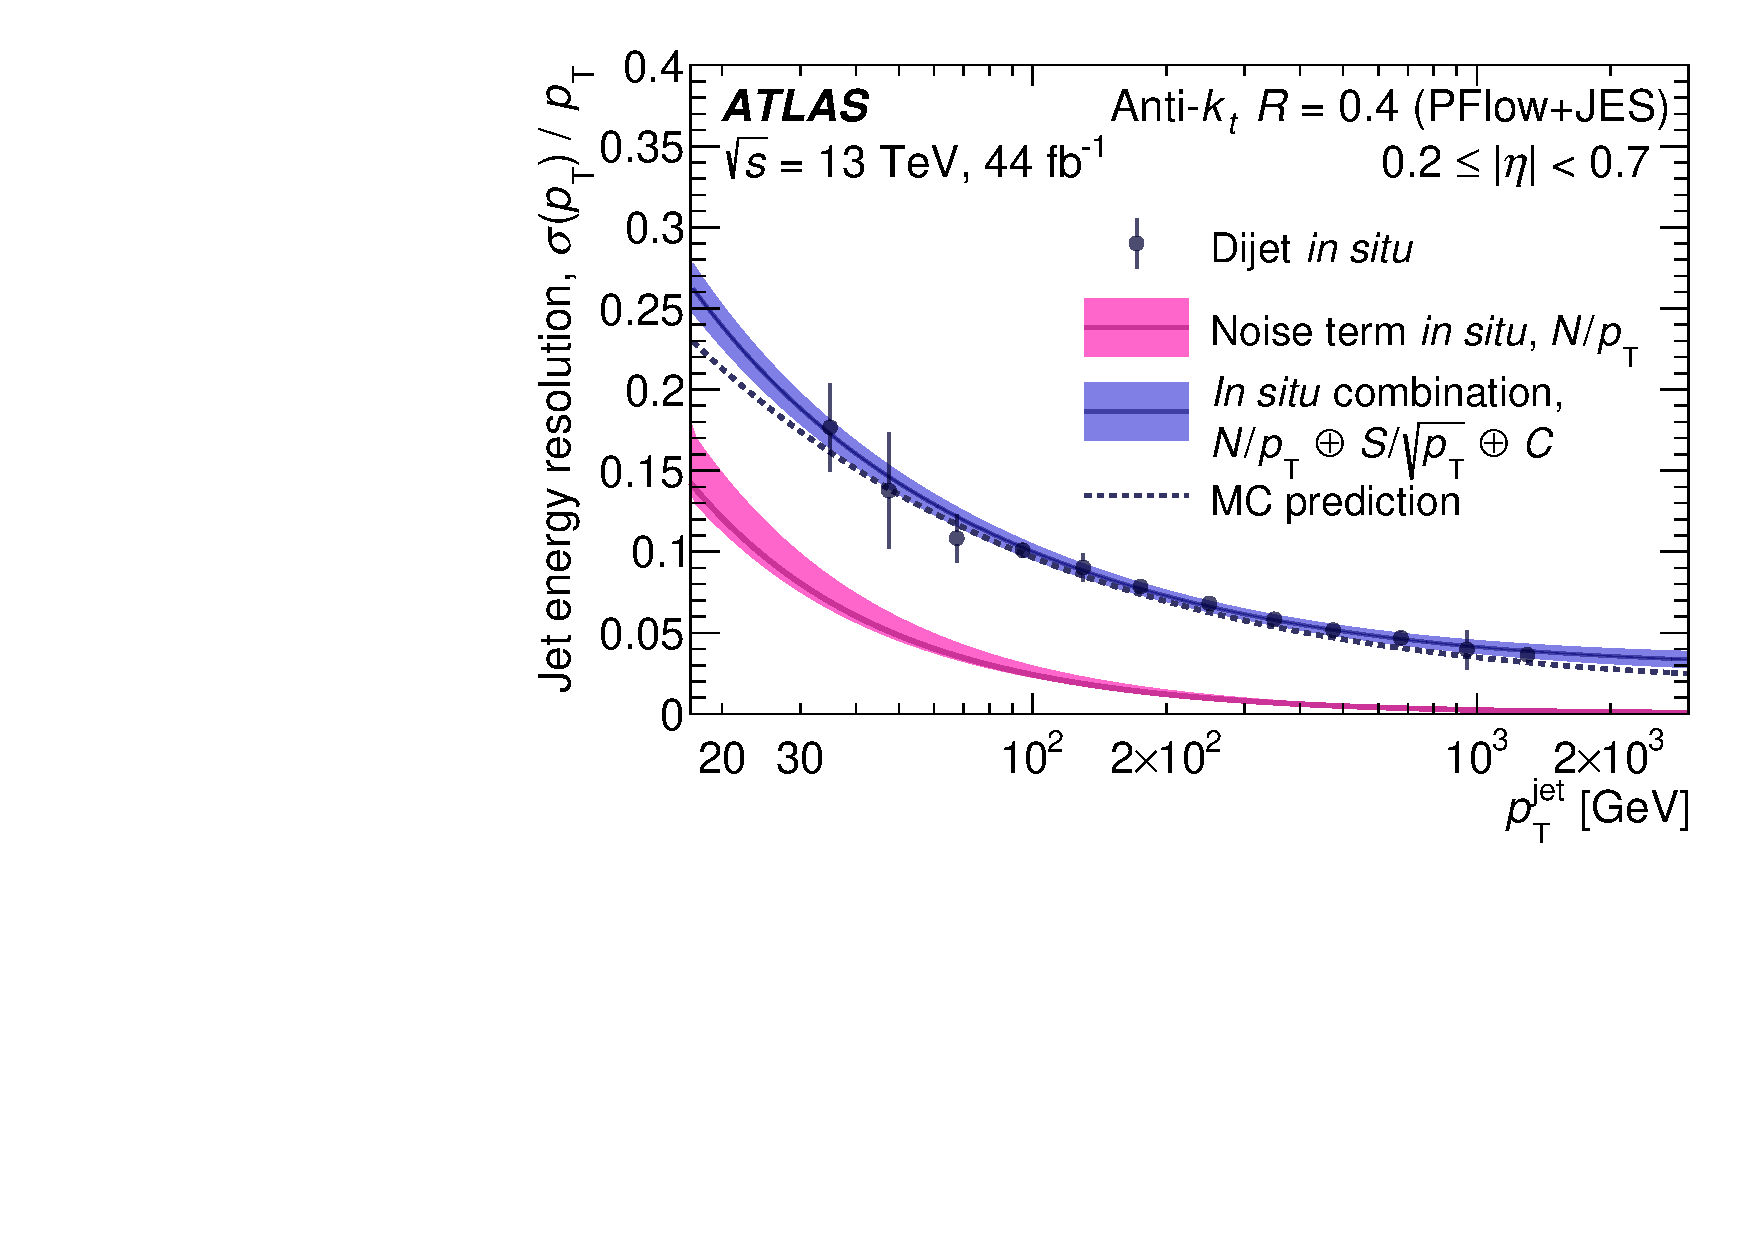
\includegraphics[width=0.495\textwidth]{jet_reso.pdf}
                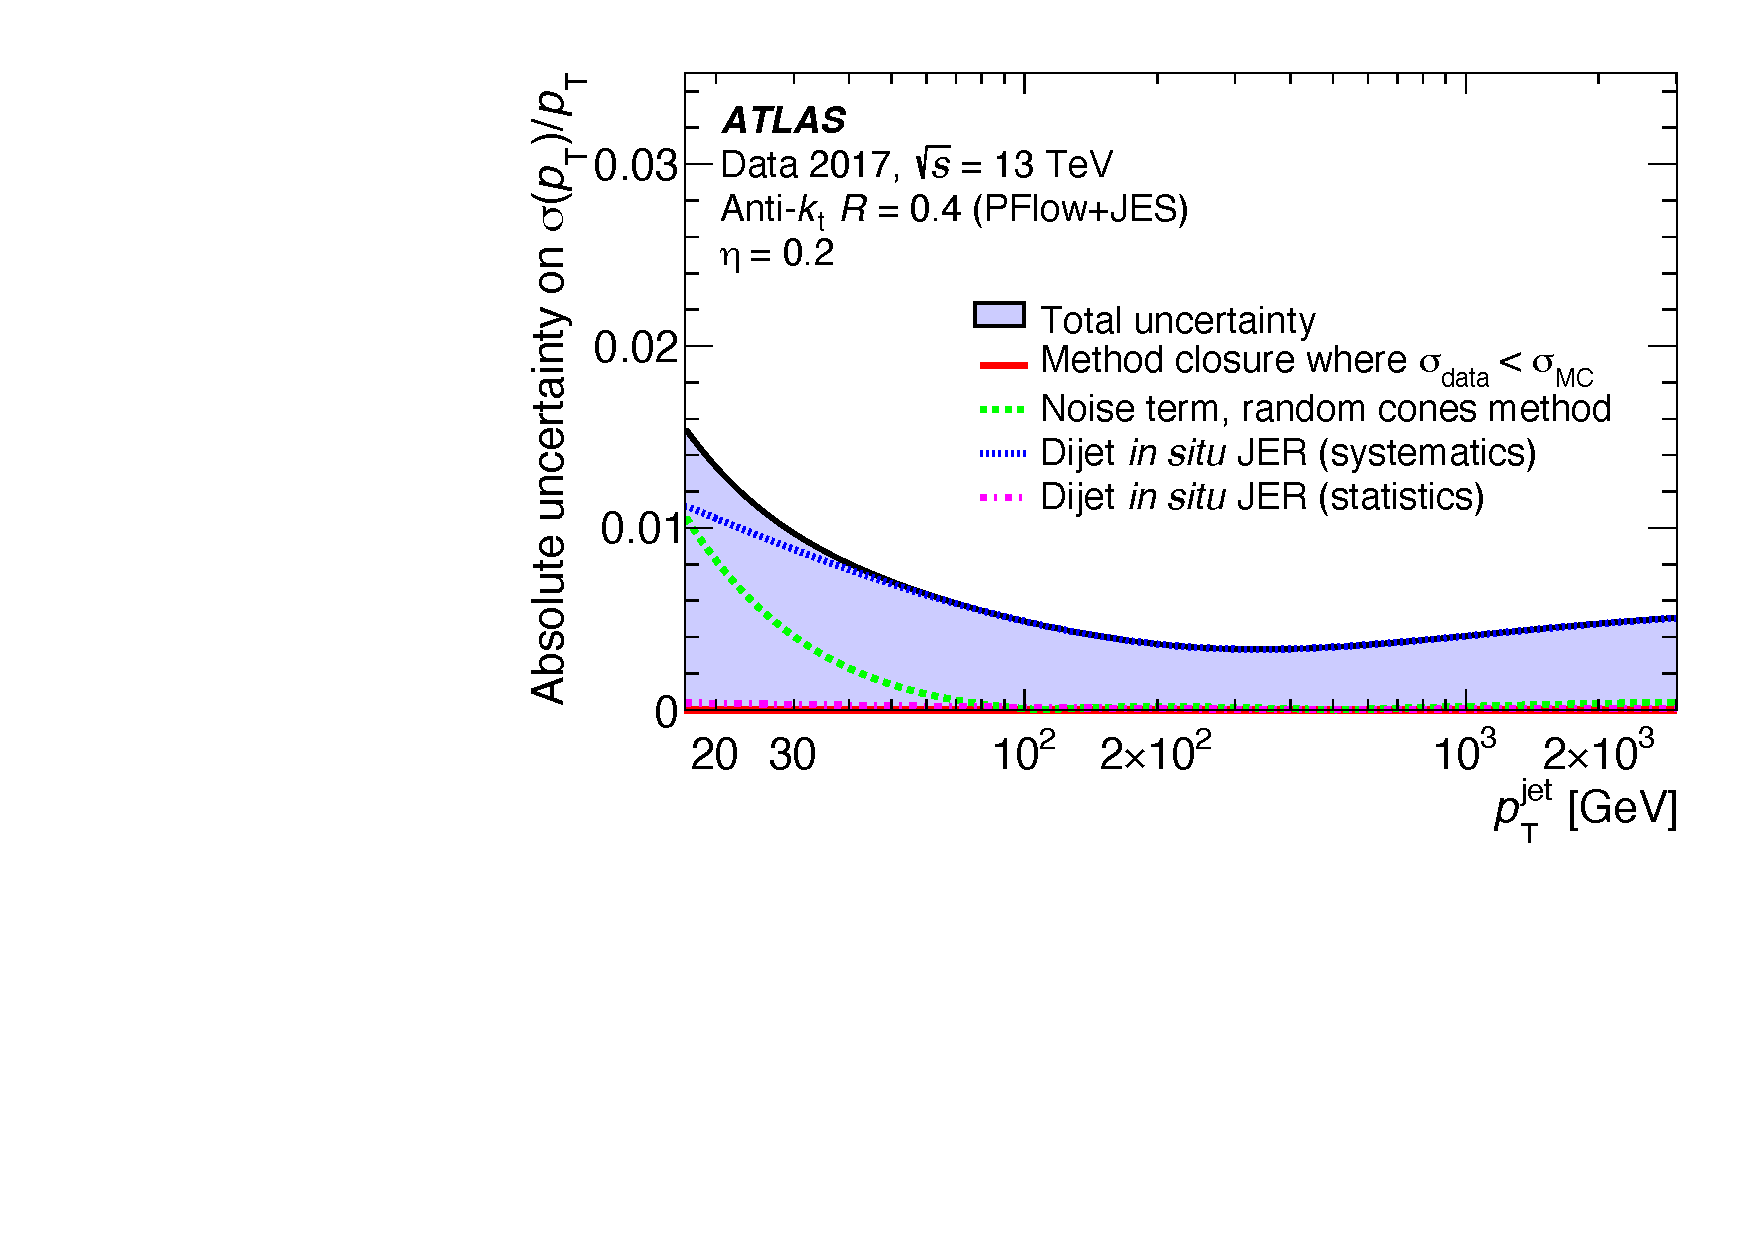
\includegraphics[width=0.495\textwidth]{jet_uncert.pdf}
                \caption{
                    (left) The relative jet energy resolution as a function of $\pt$ for fully calibrated PFlow+JES jets. 
                    The error bars on points indicate the total uncertainties on the derivation of the relative resolution in dijet events, 
                    adding in quadrature statistical and systematic components. 
                    The expectation from Monte Carlo simulation is compared with the relative resolution as evaluated in data through the combination of the dijet balance and random cone techniques. 
                    (right) Absolute uncertainty on the relative jet energy resolution as a function of jet $\pt$. 
                    Uncertainties from the two in situ measurements and from the data/MC simulation difference are shown separately.
                    These figures are taken from~\cite{JETM-2018-05}.
                }
                \label{fig:jet_reso}
            \end{figure}

        \subsubsection{Large-radius jets}
            Large-radius jets are specifically optimised to identify highly boosted topologies, particularly those involving boosted objects 
            such as \(W\), \(Z\), and Higgs bosons, as well as top quarks~\cite{JETM-2018-03}. These jets are typically reconstructed using the anti-\(k_t\) 
            algorithm with a large radius parameter (\(R = 1.0\)). The substantial radius allows the jet to capture more of the 
            radiation and decay products from highly boosted massive particles, thus providing a clearer insight into their substructure.
            In Run 2 and Run 3, the unified flow objects (UFOs)~\cite{JETM-2018-02,JETM-2018-06} have been developed to address the need for a jet input object that 
            combines desirable aspects of PFlow and Track-CaloClusters (TCC)~\cite{JETM-2018-02} reconstruction. This integration aims to further optimise 
            performance metrics, such as jet energy resolution and pile-up stability, across the full kinematic range.
            The UFO reconstruction process begins with the standard ATLAS PFlow algorithm. Charged PFlow objects (PFOs) matched 
            to pile-up vertices are removed, ensuring that only relevant tracks from the primary vertex are considered.
            The remaining PFOs are categorised into three category: neutral PFOs, charged PFOs used for subtracting energy from a topocluster,
            and charged PFOs in dense environments. In these dense environments, charged particles produced in regions is very high, 
            the detector may encounter challenges in isolating individual particle signals, and as a result, 
            no energy subtraction is performed for these PFOs.
            Jet-input-level pile-up mitigation algorithms, such as Constituent Subtraction (CS) and SoftKiller (SK)~\cite{ATLAS-CONF-2017-065}, 
            are applied to neutral PFOs to further reduce pile-up effects. A modified version of the TCC splitting algorithm is 
            then applied, using only tracks from the primary vertex to avoid pile-up instabilities. Tracks used for PFlow 
            subtraction are excluded from this step, as their contributions have already been subtracted.
            UFOs demonstrate improved tagging performance across both low and high \( p_T \) ranges, showing superiority over 
            TCC jets at high \( p_T \) and becoming comparable to PFlow jets at lower \( p_T \). Due to the inclusion of only 
            charged-particle tracks matched to the primary vertex, UFOs exhibit natural stability against pile-up, similar to 
            the PFlow algorithm. Additional stability is provided by input-level pile-up mitigation algorithms applied to neutral 
            particles. UFOs offer an improved jet mass resolution compared to existing large-\( R \) jet definitions, with up to a 
            45\% improvement at high \( p_T \) for signal jets. 
            However, the calibration process for UFOs is more complex due to the need to account for various factors such as the
            pile-up contribution and the energy scale of different components~\cite{JETM-2023-02}. 


    \subsection{Missing transverse energy (\MET) reconstruction}
        Missing transverse energy, also referred to as missing transverse momentum, serves as a proxy for the transverse momentum 
        carried by undetected particles, which can be indicative of phenomena such as neutrino production within the SM or 
        potential new physics scenarios like dark matter.
        The reconstruction of \MET~\cite{JETM-2020-03} involves the combination of multiple detector inputs, including calibrated electrons, muons, photons, hadronically decaying 
        \(\tau\)-leptons, hadronic jets, and soft activity from remaining tracks. This process is inherently complex due to the need to avoid double-counting 
        of momentum and to accurately represent the event's transverse momentum balance.
        \subsubsection{\MET reconstruction}
            The reconstruction process of \MET in ATLAS is divided into two main components:
            \begin{itemize}
                \item Hard Term (\(p_T^{\text{hard}}\)): This includes signals from well-reconstructed and calibrated hard objects such as electrons, 
                photons, \(\tau\)-leptons, muons, and jets. Each of these objects is carefully selected and calibrated to ensure accurate measurement.
                \item Soft Term (\(p_T^{\text{soft}}\)): This consists of contributions from tracks associated with the primary interaction vertex but not 
                associated with any hard object. The soft term helps capture the residual transverse momentum in the event that is not accounted for by the hard objects.
            \end{itemize}
            To form the \MET vector, these components are combined as follows:
            \[ 
            \vec{E}_T^{\text{miss}} = - \left( \sum \vec{E}_T^{\text{hard}} + \sum \vec{E}_T^{\text{soft}} \right)
            \]
            where the sums run over all selected hard objects and soft tracks, respectively.
            One of the key challenges in \MET reconstruction is avoiding double counting of detector signals. This is managed through a signal ambiguity resolution 
            procedure that ensures each detector signal contributes to only one hard object. The procedure priorities signals by a set of criteria, detailed in~\cite{olr:exact}
        \subsubsection{\MET calibration}
            ATLAS has defined several \MET working points, each with varying levels of stringency on jet selections to manage pile-up and other sources of fake 
            \MET. These working points range from loose to tenacious, with the latter offering the highest resilience to pile-up by applying more stringent 
            requirements on jets, particularly in the forward region of the detector.
            The performance of \MET reconstruction is evaluated using both real data and MC simulations. The key metrics for performance include 
            the resolution of \MET and its systematic uncertainties. The resolution is typically assessed in events with well-known kinematic properties, such 
            as \(Z \rightarrow \ell^+\ell^-\) decays, which provide a clean sample with no true \MET.
            The adoption of a particle flow algorithm, which combines calorimeter and tracking information, improves the resolution of jets. 
            This, in turn, facilitates dynamic \MET reconstruction that adapts based on the chosen hard objects in an analysis.
            Systematic uncertainties are thoroughly evaluated for both the hard and soft components of \MET. Recent studies have shown significant 
            reductions in scale and resolution uncertainties, thanks to improved calibration techniques and better handling of pile-up effects.
            \begin{figure}[htbp]
                \centering
                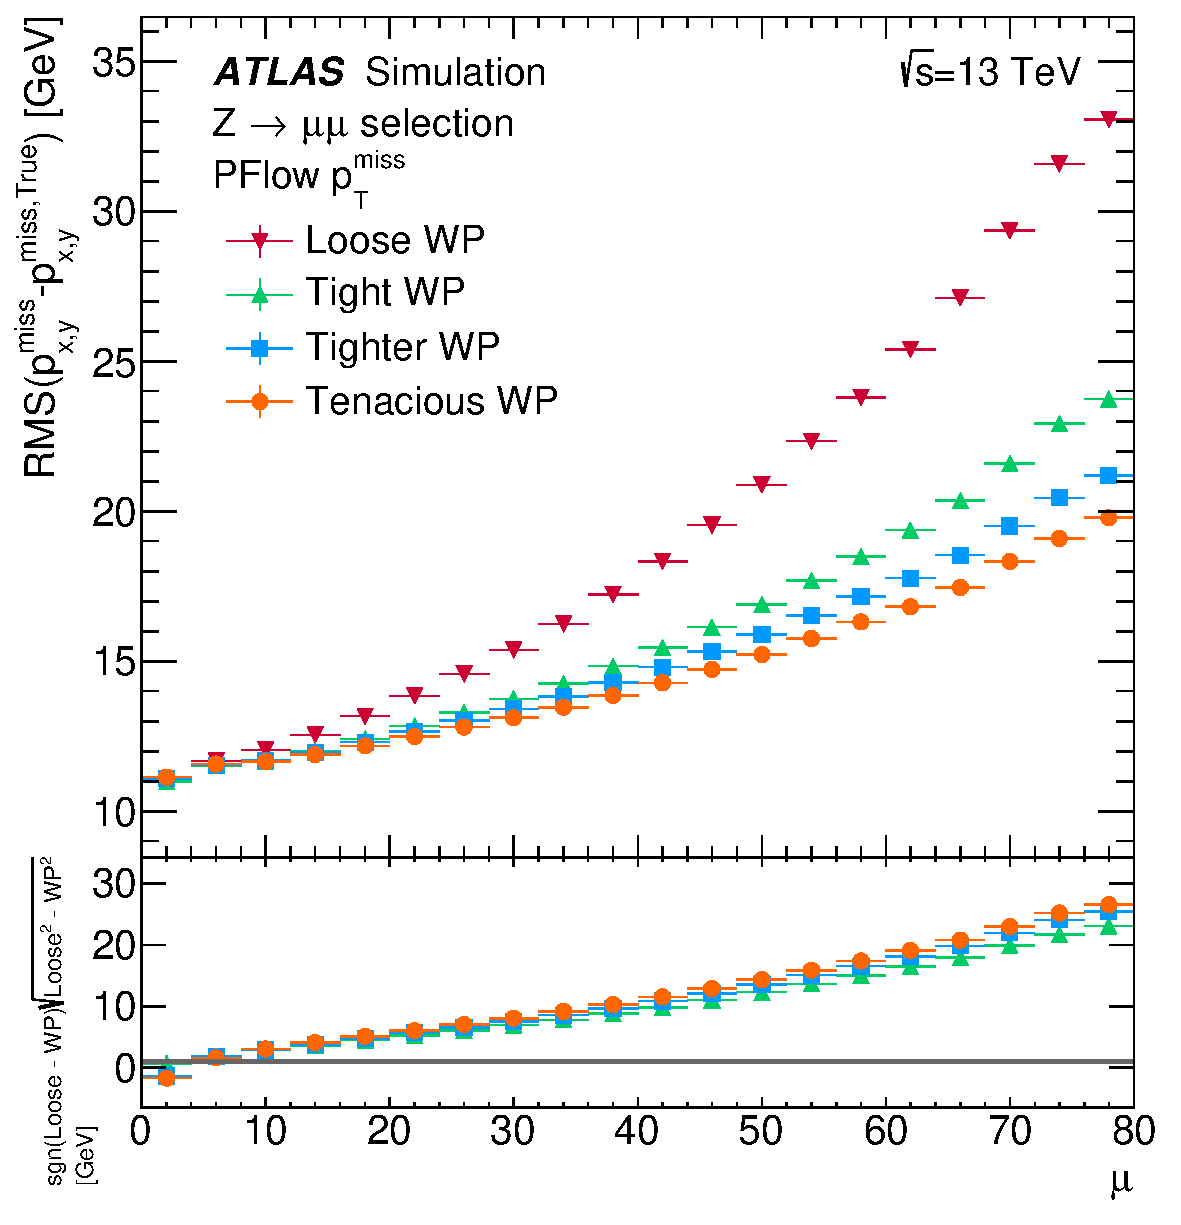
\includegraphics[width=0.495\textwidth]{met_reso_mu.pdf}
                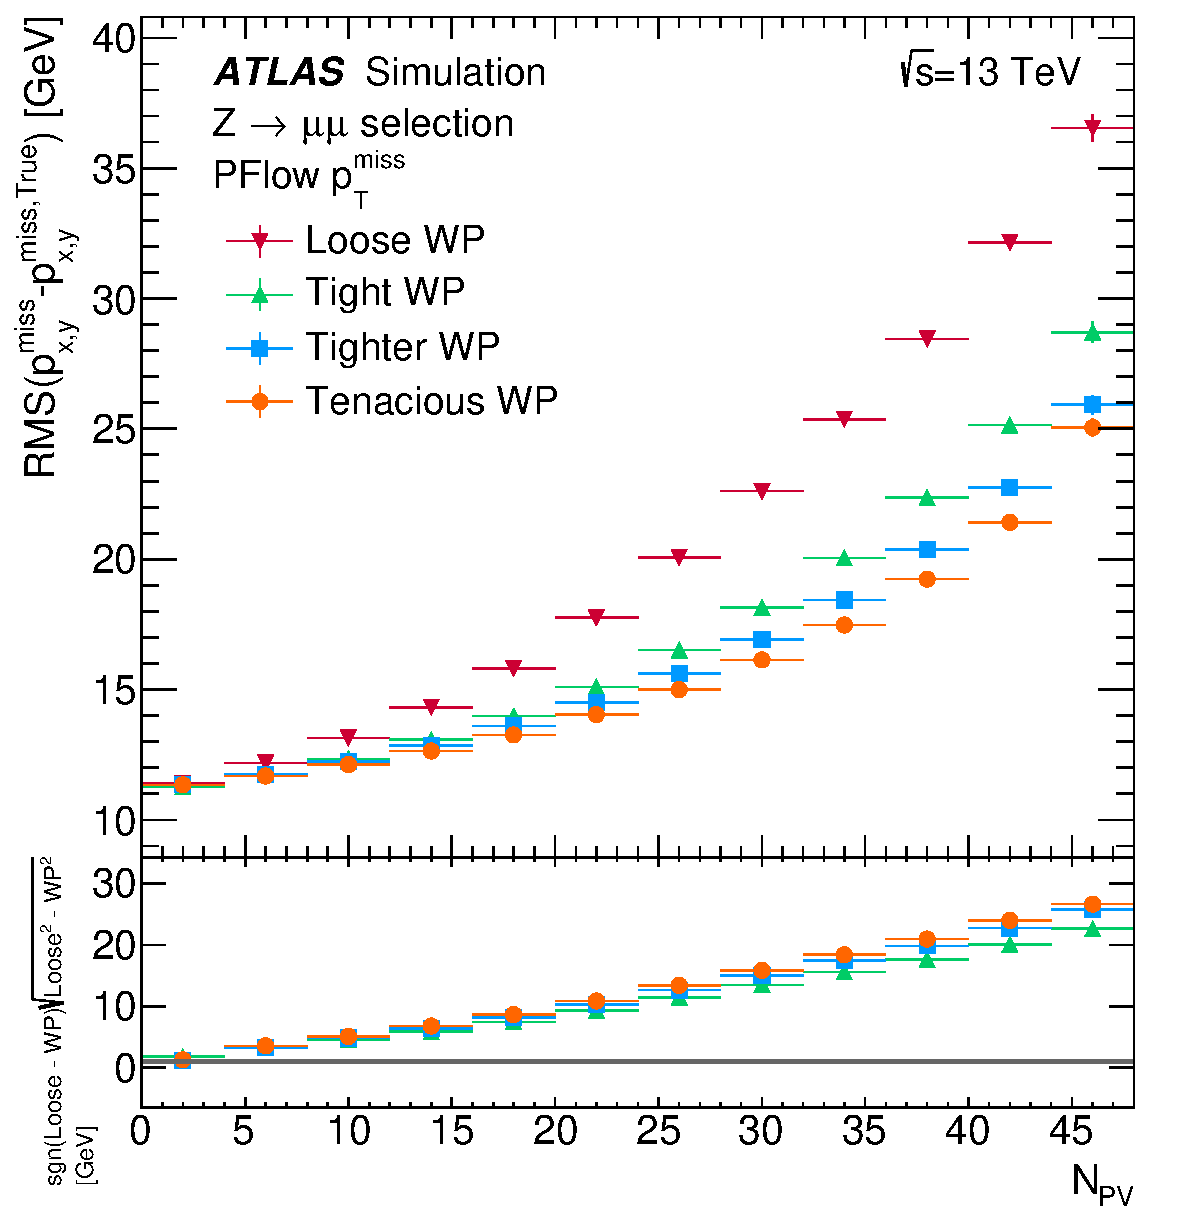
\includegraphics[width=0.495\textwidth]{met_reso_pv.pdf}
                \caption{
                    The $p_x^\text{miss}$ and $p_y^\text{miss}$ resolution for different $p_\text{T}^\text{miss}$ working points as a function of interactions per bunch crossing (left) or number of primary vertices (right). 
                    PFlow jets are used on SM MC simulations with $Z\rightarrow\mu\mu$ events. 
                    These figures are taken from~\cite{JETM-2020-03}.
                }
                \label{fig:met_reso}
            \end{figure}

            
    

    \subsection{Jet flavour tagging}
        The ATLAS experiment employs a sophisticated array of algorithms for identifying jets containing \(b\)-hadrons (b-jets) and \(c\)-hadrons (c-jets), 
        commonly referred to as flavour-tagging algorithms~\cite{FTAG-2019-07,ATL-PHYS-PUB-2022-027}. The core of these algorithms lies in exploiting the unique characteristics of \(b\)- and \(c\)-hadrons, 
        such as their long lifetimes, high masses, and complex decay patterns, to distinguish them from jets originating from lighter quarks. Specialised 
        flavour tagging is also designed to identify large-radius jets originating from boosted Higgs bosons decaying into pairs of bottom quarks (\(H \to b\bar{b}\)) 
        and charm quarks (\(H \to c\bar{c}\))~\cite{ATL-PHYS-PUB-2020-019,ATL-PHYS-PUB-2023-021}. The latest developments in jet flavour tagging employ Graph Neural Networks
        to enhance performance~\cite{ATL-PHYS-PUB-2022-027, ATL-PHYS-PUB-2023-021}.

        \subsubsection{DL1r taggers}
            The Run 2 flavour-tagging strategy of ATLAS is based on a two-stage approach. The first stage involves low-level taggers that reconstruct specific 
            features of heavy-flavour jets using two complementary methods: track-based and vertex-based approaches. Track-based algorithms analyse the 
            properties of individual charged-particle tracks associated with a hadronic jet, while vertex-based algorithms focus on reconstructing displaced 
            vertices from these tracks. Key low-level taggers include:
            \begin{itemize}
                \item Impact Parameter Algorithms (IP2D, IP3D)~\cite{ATL-PHYS-PUB-2017-013}: These algorithms utilise the impact parameters of tracks, which are the distances of 
                closest approach of tracks to the primary vertex. IP2D and IP3D calculate likelihood ratios from the track impact parameter significances, 
                with IP3D additionally considering the 3D impact parameter.
                \item Secondary Vertex Finder (SV1)~\cite{ATL-PHYS-PUB-2017-011}: This algorithm reconstructs secondary vertices within the jet by combining tracks that originate 
                from a common point away from the primary collision vertex. It enhances pile-up rejection and overall performance at high jet \( p_T \) through 
                advanced track-cleaning and vertexing techniques.
                \item JetFitter~\cite{ATL-PHYS-PUB-2018-025}: This algorithm aims to reconstruct the entire decay chain of \(b\)-hadrons within the jet by employing a topological 
                vertex finding approach. It identifies multiple vertices and uses a Kalman filter to improve vertex reconstruction.
                \item RNNIP: A track-based Recurrent Neural Network (RNN) that utilises the sequential nature of track hits to improve the identification 
                of \(b\)- and \(c\)-jets.
            \end{itemize}
            The outputs of the low-level taggers are then fed into high-level taggers, which are multivariate classifiers designed to maximise 
            flavour-tagging performance. The primary high-level tagger used during Run 2 is the DL1~\cite{ATL-PHYS-PUB-2017-013} algorithm series, which employs deep learning techniques.
            DL1 Combines the outputs of IP2D, IP3D, SV1, and JetFitter using a feed-forward neural network.
            DL1r~\cite{ATL-PHYS-PUB-2017-013}is an enhanced version of DL1 that also incorporates the RNNIP outputs. DL1r significantly improves the tagging performance by 
            leveraging the low correlation of RNNIP outputs with other taggers.
            The performance of flavour-tagging algorithms is evaluated in terms of their efficiency to correctly identify \(b\)-jets (\(\epsilon_b\)) 
            and their ability to reject light-flavour jets and \(c\)-jets. The DL1d tagger achieves a light-flavour jet rejection factor of 170 and 
            a charm-jet rejection factor of 5 at a \(b\)-jet identification 
            efficiency of 77\%. For charm-jet identification, DL1r achieves a light-flavour jet rejection factor of 70 and a \(b\)-jet rejection 
            factor of 9 at a charm-jet efficiency of 30\%. The flavour-tagging performance is further assessed across various jet \(p_T\) and \(|\eta|\) 
            ranges, and by ensuring robustness against pile-up interactions. The algorithms maintain consistent performance even with increased pile-up, 
            showing minimal variation in \(b\)-tagging efficiency and background rejection factors across different collision environments.
        
        \subsubsection{GNN-based tagger}
            In Run-3, ATLAS will implement a novel jet tagger using a Graph Neural Network (GNN) architecture known as GN1~\cite{ATL-PHYS-PUB-2022-027, ATL-PHYS-PUB-2023-021}. This advanced method 
            represents a significant departure from traditional flavour tagging approaches, relying on its ability to process information from a 
            variable number of charged particle tracks within a jet without intermediate low-level algorithms. Here, we detail the architecture, 
            implementation, and performance of the GNN-based taggers.
        
            GN1 utilises a sophisticated GNN layer combined with auxiliary training objectives. The primary goal is jet flavour 
            classification, identifying whether jets originate from \(b\)- or \(c\)-quarks. GN1 employs a fully connected graph where each node 
            represents a track within the jet. These nodes are characterised by feature vectors derived from a per-track initialisation network, 
            which then interact within the graph to predict jet flavour, track origins, and vertex groupings. 
            GN1 demonstrates superior performance compared to the current DL1r tagger across various metrics. For jets within the \(t\bar{t}\) 
            sample with transverse momentum (\(p_T\)) between 20 and 250 GeV, GN1 improves light-jet and \(c\)-jet rejection by factors of 
            approximately 1.8 and 2.1, respectively, at a 70\% \(b\)-jet tagging efficiency. In the higher \(p_T\) range (250 < \(p_T\) < 5000 GeV) 
            from the \(Z'\) sample, these improvements rise to factors of around 6 for light-jet rejection and 2.8 for \(c\)-jet rejection at a \(b\)-jet efficiency of 30\%.
            This method's inclusive reconstruction efficiency in \(b\)-jets reaches approximately 80\%, indicating its robust capability to 
            identify displaced vertices from \(b\)-hadron decays.
            GN1 represents a significant advancement in jet flavour tagging for the ATLAS experiment, offering improved performance and flexibility. 
            By eliminating the dependence on low-level algorithms and employing a unified GNN approach, GN1 not only enhances the efficiency of 
            \(b\)- and \(c\)-jet identification but also simplifies the optimisation process for various tagging applications.
            \begin{figure}[htbp]
                \centering
                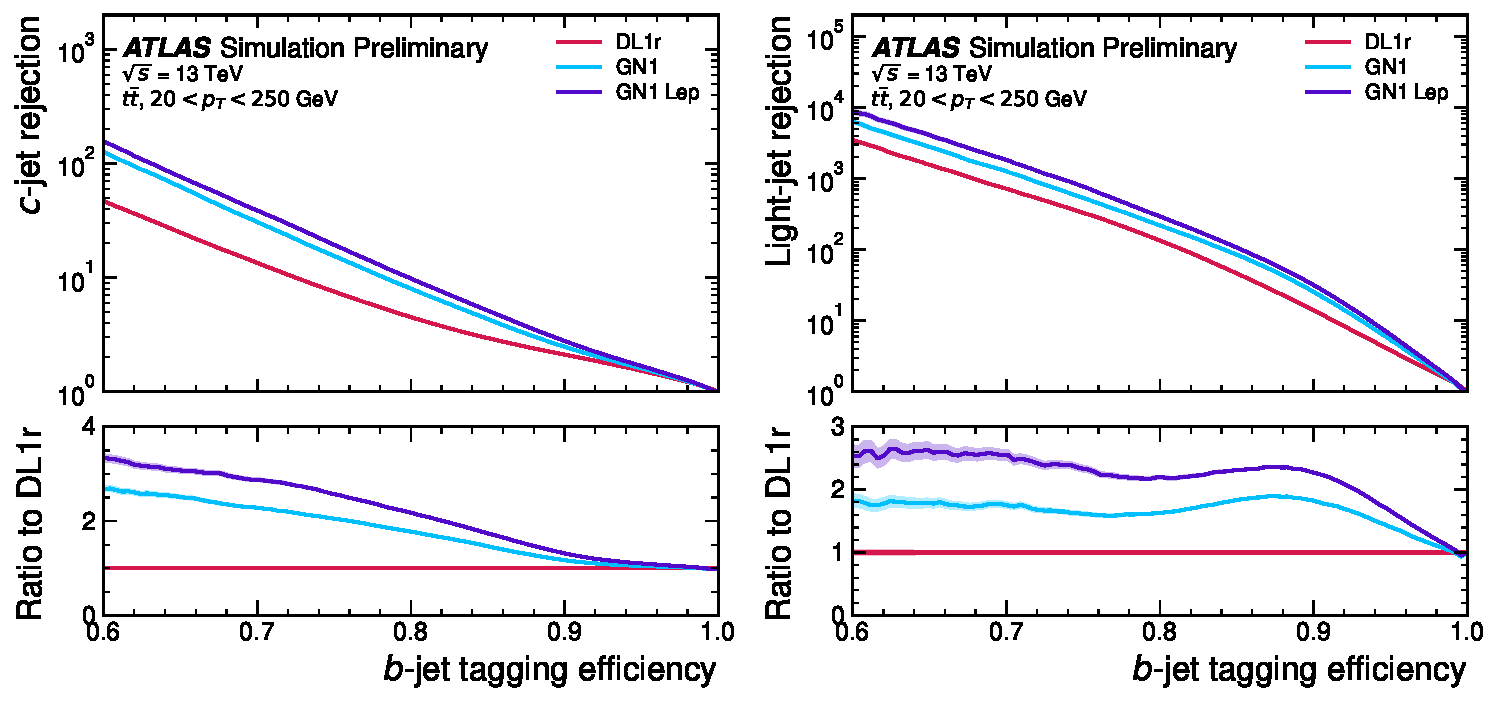
\includegraphics[width=1.0\textwidth]{GN2_roc.pdf}
                \caption{
                    The GN2 c-jet (left) and light-jet (right) rejections as a function of the b-jet tagging efficiency for jets in the $\ttbar$ sample with $20 < \pT < 250$ GeV. 
                    The ratio with respect to the performance of the DL1r algorithm is shown in the bottom panels. 
                    These figures are taken from~\cite{ATL-PHYS-PUB-2022-027}.
                }
                \label{fig:GN2_roc}
            \end{figure}
        
        \subsubsection{GNN-based flavour tagging for large-R jets}
            In Run 3, ATLAS advanced its flavour tagging capabilities with the development of the GN2X~\cite{ATL-PHYS-PUB-2023-021} algorithm, designed to 
            identify large-radius jets originating from boosted Higgs bosons decaying into pairs of bottom quarks (\(H \to b\bar{b}\)) and charm quarks 
            (\(H \to c\bar{c}\)). The GN2X algorithm leverages recent advancements in GNNs and transformer architectures, 
            providing significant improvements in background rejection and tagging efficiency compared to previous methods.
            
            The base GN2X model takes three large-radius jet variables and 20 track variables as inputs. Up to 100 tracks per 
            jet are considered, sorted by decreasing transverse impact parameter significance to prioritise tracks from displaced vertices.
            The GN2X architecture utilises a transformer network with multiple encoder blocks and attention 
            heads~\cite{shleifer2021normformerimprovedtransformerpretraining, ba2016layernormalization} to process the track 
            representations. This setup allows the model to capture complex relationships among tracks and derive a global jet representation for classification.
            In addition to the primary jet classification task, GN2X includes auxiliary training objectives for track origin 
            classification and vertex grouping, enhancing the model's ability to identify displaced vertices and improve tagging performance.
            GN2X achieves significant improvements in background rejection compared to previous taggers in \(H \to b\bar{b}\) tagging. At a 
            50\% \(H(b\bar{b})\) tagging efficiency, GN2X provides a background rejection factor of 40 for jets from top quark decays and 300 
            for multijet events. This represents a factor of 1.6 improvement in top jet rejection and a factor of 2.5 improvement in multijet 
            rejection compared to the baseline tagger $D_\mathrm{xbb}$~\cite{FTAG-2019-07}.
            For \(H(c\bar{c})\) tagging, GN2X offers substantial enhancements in rejecting background jets, including those from \(H(b\bar{b})\) 
            decays. At a 50\% \(H(c\bar{c})\) tagging efficiency, GN2X achieves a factor of 3 improvement in top jet rejection, 
            a factor of 5 improvement in multijet rejection, and a factor of 6 improvement in \(H(b\bar{b})\) rejection.
            GN2X maintains stable tagging efficiency across the entire transverse momentum (\(p_T\)) spectrum of the jets. At a 50\% 
            \(H(b\bar{b})\) efficiency working point, GN2X shows consistent performance, significantly outperforming the baseline taggers 
            across all \(p_T\) ranges. The algorithm exhibits less efficiency drop-off at high \(p_T\) compared to previous methods, 
            ensuring reliable performance even for high-energy jets.
            \begin{figure}[htbp]
                \centering
                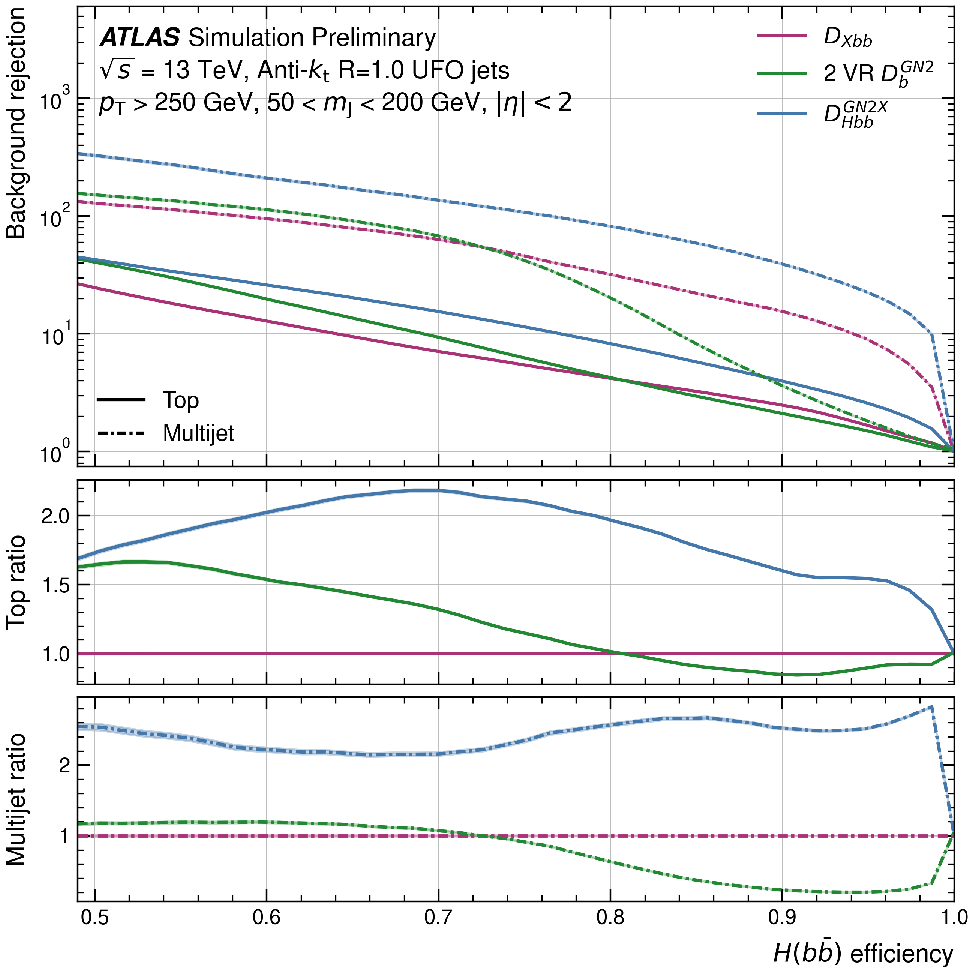
\includegraphics[width=0.5\textwidth]{GN2x_roc.pdf}
                \caption{
                    GN2x top and multijet rejections as a function of the $H\rightarrow bb$ efficiency for jets with $\pt>250$ GeV and mass ($50~\GeV < m_J < 200~\GeV$). 
                    Performance of the GN2X algorithm is compared to the previous DXbb tagger and variable-radius subjets baselines.
                    These figures are taken from~\cite{ATL-PHYS-PUB-2023-021}.
                }
                \label{fig:GN2x_roc}
            \end{figure}


    \subsection{Muon reconstruction and identification}
        The muon reconstruction and identification process~\cite{MUON-2018-03} involves several sophisticated techniques that use the 
        capabilities of the ATLAS detector's subsystems, including the Inner Detector (ID), Muon Spectrometer (MS), 
        and calorimeters.
        
        \subsubsection{Muon reconstruction}
            Muon reconstruction in ATLAS primarily exploits the characteristics of minimum-ionising particles. This involves the identification of 
            tracks within the MS or through specific energy deposits in the calorimeters. The reconstruction process utilises data from both the 
            ID and MS tracking detectors, with calorimeter information contributing to track parameter determination and tagging of muon candidates 
            independently from the MS.
        
            The MS Stand-Alone Reconstruction process starts by identifying short straight-line segments from hits in individual MS stations using 
            a Hough transform. These segments are combined into track candidates, taking into account the initial pointing constraint and the 
            parabolic trajectory of the muon bending in the magnetic field. A global $\chi^2$ fit of the muon trajectory is then performed, 
            which considers possible interactions with detector material and misalignments between detector chambers. Outliers are removed, 
            and missing hits are added to refine the track fit. The final track is extrapolated back to the beam line, with its \pT expressed 
            at the interaction point (IP). Global Muon Reconstruction involves a combination of information from the ID, MS, and calorimeters. 
            The process follows five main strategies, resulting in different types of muons: Combined (CB), Inside-Out (IO), Muon-Spectrometer 
            Extrapolated (ME), Segment-Tagged (ST), and Calorimeter-Tagged (CT)~\cite{MUON-2018-03}. Each type has its reconstruction pathway, which includes 
            matching MS tracks to ID tracks, extrapolating ID tracks to the MS, or using calorimeter data to tag muons.
        
        \subsubsection{Muon identification}
            Different WPs are defined based on the required efficiency, resolution, and background rejection. These criteria are applied to hits 
            in the ID and MS, track fit properties, and compatibility variables between detector measurements. The WPs are tailored to optimise 
            performance for various physics analyses, targeting prompt-muon identification, momentum resolution, and non-prompt muon rejection.
            The tag-and-probe method uses dimuon pairs from $Z\rightarrow \mu^+\mu^-$ decays to measure reconstruction and identification 
            efficiencies. One muon (the tag) must satisfy stringent criteria and trigger the event-selection, while the other (the probe) tests 
            the efficiency of specific algorithms. Several probe types (ID, MS, CT, ST) are used to measure various efficiencies, and a matching 
            requirement of $\Delta R < 0.05$ is applied to ensure accurate efficiency measurements. Efficiency scale factors are derived to correct 
            simulation data to match real detector performance.
            \begin{figure}[htbp]
                \centering
                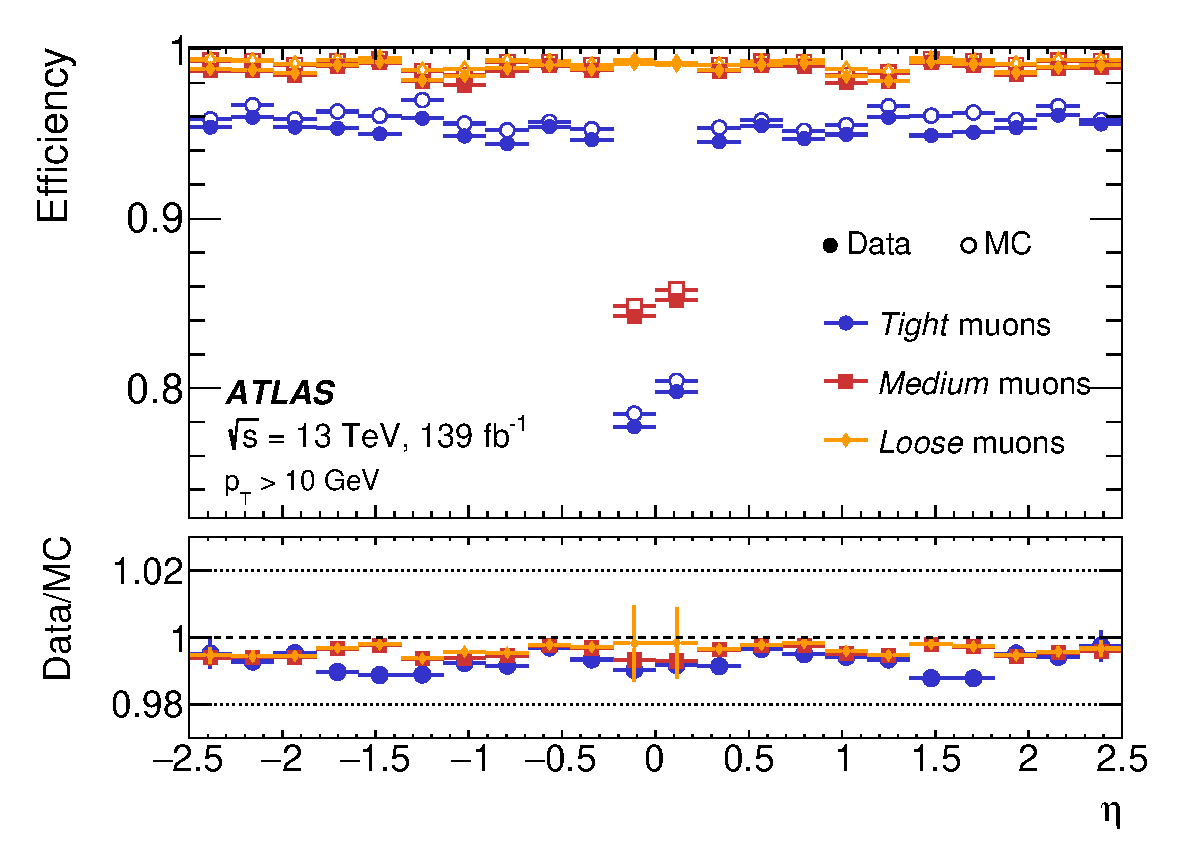
\includegraphics[width=0.6\textwidth]{muon_effi_eta.pdf}
                \caption{
                    Muon reconstruction and identification efficiencies for the Loose, Medium, and Tight criteria. It displays the efficiencies measured in $Z\rightarrow\mu\mu$ events as a function of $\eta$, for muons with $\pt>10$~GeV. 
                    This figure is taken from~\cite{MUON-2018-03}.
                }
                \label{fig:muon_effi}
            \end{figure}
        
        \subsubsection{Muon calibration}
            Muon momentum calibration~\cite{MUON-2022-01} is critical for achieving precise measurements, especially given the complexities of the detector geometry and alignment.
            Biases introduced by residual misalignments in the detector are corrected using a charge-dependent momentum calibration technique. This method
            involves analysing the mass of the dimuon system from Z$\rightarrow \mu^+\mu^-$ decays to estimate and correct biases in the muon momentum
            scale. The calibration procedure is validated using independent samples of J/$\psi\rightarrow\mu^+\mu^-$ and $\Upsilon\rightarrow\mu^+\mu^-$ decays.
            These procedures include detailed studies of detector response, alignment system uncertainties, and the development of correction factors for both the ID and MS.
            The ultimate goal is to minimise the systematic uncertainties and achieve the highest possible precision in momentum measurement.
        
    \subsection{$\tau$ lepton reconstruction}
        A $\tau$ lepton has a 35\% probability of decaying leptonically to a lighter lepton ($\tau_\mathrm{e}$ or $\tau_\mathrm{\mu}$) and two neutrinos. 
        In the remaining 65\% of cases a $\tau$ lepton decays hadronically ($\tauhad$) to one or more charged hadrons, zero or more
        neutral hadrons, plus one neutrino. 
        The leptonically decaying $\tau$ leptons are reconstructed as prompt electrons or muons in the ATLAS detector with non-zero impact parameters. 
        The visible part of the hadronically decaying $\tau$ leptons ($\tauhadvis$) are reconstructed and identified using a combination of tracking and calorimetric information. 

        A significant portion of this thesis is dedicated to the detailed reconstruction and identification of $\tauhadvis$. 
        This constitutes a major part of the research I have been worked on. 
        The next chapter will delve deeply into this topic, providing comprehensive insights and methodologies.